\documentclass{experimentreport}

\usepackage{listings}
\usepackage{xcolor}

\definecolor{codegreen}{rgb}{0,0.6,0}
\definecolor{codegray}{rgb}{0.5,0.5,0.5}
\definecolor{codepurple}{rgb}{0.58,0,0.82}
\definecolor{backcolour}{rgb}{0.95,0.95,0.92}
\definecolor{lightgreen}{rgb}{0,0.4,0}
\definecolor{lightred}{rgb}{0.4,0,0}

\definecolor{mygray}{gray}{.9}

% \lstdefinestyle{mystyle}{
\lstset{
    %backgroundcolor=\color{backcolour},   
    commentstyle=\color{brown},
    keywordstyle=\color{magenta},
    numberstyle=\tiny\color{codegray},
    stringstyle=\color{codepurple},
    basicstyle=\ttfamily\tiny,
    breakatwhitespace=false,         
    breaklines=true,                 
    captionpos=b,                    
    keepspaces=true,                 
    numbers=none,                    
    numbersep=5pt,                  
    showspaces=false,                
    showstringspaces=false,
    showtabs=false,                  
    tabsize=2,
    escapeinside={<@}{@>}
}

% \lstset{
% basicstyle=\ttfamily\bfseries\footnotesize,
%   morekeywords={virtualinvoke},
%   keywordstyle=,
%   ndkeywordstyle=\color{red},
%   commentstyle=\color{gray},
%   stringstyle=\color{green},
%   numbers=none,
%   breaklines=true,
%   numberstyle=\ttfamily\footnotesize\color{gray},
%   stepnumber=1,
%   numbersep=6pt,
%   backgroundcolor=\color{white},
%   tabsize=4,
%   showspaces=false,
%   showstringspaces=false,
%   xleftmargin=6pt,
%   captionpos=t
% }

\lstdefinelanguage{JavaScript}{
  keywords={typeof, new, true, false, catch, function, return, null, catch, switch, var, if, in, while, do, else, case, break, export, static, const, let, class, void, async, await, interface, extends, public, this},
  % basicstyle=\linespread{1.0}\ttfamily\footnotesize,
  % keywordstyle= \color{violet}\bfseries,
  ndkeywords={class, export, boolean, throw, implements, import, this},
  ndkeywordstyle=\color{darkgray}\bfseries,
  identifierstyle=\color{black},
  sensitive=false,
  frame=lines,
  comment=[l]{//},
  morecomment=[s]{/*}{*/},
  % commentstyle=\color{gray}\ttfamily,
  % stringstyle=\color{blue}\ttfamily,
  morestring=[b]',
  morestring=[b]"
}



\usepackage{graphicx}
\usepackage{hyperref}
\usepackage{enumitem}
\usepackage{amsmath}
\usepackage{booktabs}
\usepackage{multirow}

%========================
% 基本信息
%========================

\setcoursename{基础软件开发技术实践}
\setreportname{智能软件工程实验报告}

\setexperimenttitle{实验二：基于机器学习的人类编写代码的代码审查}

\setstudentname{\hintholder{廖正强}}
\setdepartment{\hintholder{计算学部}}
\setstudentid{\hintholder{2023112920}}

\setcourseteacher{刘佳琨}
\setinstructor{刘佳琨}

\setlablocation{\hintholder{格物213}}
\setlabtime{    \hintholder{2026/7/6}}

\begin{document}

%========================
% 自动生成封面
%========================

\makereporthead

%========================
% 实验目的
%========================

\experimentpurpose{

本实验是"代码审查"研究系列的第二个实验，在实验一构建的 GitHub Pull Request 数据集基础上，使用传统机器学习方法完成 Merge Prediction 任务。

具体目标包括：
\begin{enumerate}[label=(\arabic*)]
    \item 从实验一数据集中筛选人类编写代码对应的 Pull Request，完成数据清洗；
    \item 生成代码中间表示，包括抽象语法树（AST）和控制流图（CFG）；
    \item 提取代码结构特征、代码修改特征、文本特征和统计特征，构建特征向量；
    \item 训练支持向量机（SVM）和随机森林（Random Forest）分类模型，预测 PR 是否会被合并；
    \item 采用 Accuracy、Precision、Recall、F1-score、ROC-AUC 等指标评估模型性能；
    \item 分析 Random Forest 特征重要性，并完成消融实验；
    \item 为后续深度学习和大语言模型实验建立传统机器学习基线。
\end{enumerate}

}

%========================
% 实验内容
%========================

\experimentcontent{

\subsection*{2.1 数据筛选与清洗}

实验一数据集包含 1500 条 PR，其中 97 条被标记为 AI 生成代码（\texttt{has\_ai\_generated\_code = True}），不满足"人类编写代码"的实验要求，予以删除。AI Reviewer 标记的 PR（431 条）予以保留，因为审查者为 AI 不代表代码本身由 AI 生成。清洗过程还包括：

\begin{itemize}
    \item 保留 \texttt{merge\_status} 为 \texttt{merged} 或 \texttt{closed\_not\_merged} 的样本；
    \item 删除 \texttt{num\_changed\_files <= 0} 的异常样本（6 条）；
    \item 文本缺失值（title、body、commit\_messages）用空字符串填充；
    \item 数值字段统一为非负数。
\end{itemize}

筛选后得到 \textbf{1397 条人类代码 PR}，合并率 63.78\%（891 条合并，506 条未合并）。

\subsection*{2.2 数据集划分}

为支持后续实验三至七的公平对比，本实验输出统一的 train/val/test 划分文件。采用分层抽样策略：

\begin{itemize}
    \item 比例：train 70\%（977 条）、val 15\%（210 条）、test 15\%（210 条）；
    \item 分层键：\texttt{repo + is\_merged}，确保每个仓库在三个子集中均有出现，且合并率分布一致；
    \item 随机种子：42。
\end{itemize}

三个子集的合并率分别为 63.77\%、63.33\%、64.29\%，与整体合并率（63.78\%）高度一致。

\subsection*{2.3 Patch 索引与代码行提取}

从实验一的 \texttt{merged\_raw.json} 中提取每个 PR 的文件级 Unified Diff Patch，按 \texttt{pr\_id} 与人类代码数据集对齐（匹配率 100\%）。

\textbf{Patch 覆盖率：}
\begin{itemize}
    \item PR 级：1395/1397（99.86\%），仅 2 条 PR 无任何 patch；
    \item 文件级：30778/31817（96.73\%）；
    \item 总计新增代码行：约 225 万行；
    \item 主要文件扩展名：\texttt{.go}（8344）、\texttt{.js}（4923）、\texttt{.md}（4810）、\texttt{.ts}（3049）、\texttt{.py}（2035）。
\end{itemize}

仅对代码文件（\texttt{.py/.go/.js/.jsx/.ts/.tsx/.java/.c/.cpp/.rs} 等）进行 AST/CFG 构建，配置、文档等非代码文件仅做统计。

\subsection*{2.4 AST 提取}

\textbf{主方案：tree-sitter。} 成功安装了 tree-sitter 及 4 种语言包（Python、JavaScript、TypeScript、Go），覆盖 P0 语言（\texttt{.py/.go/.js/.ts/.tsx}）。使用 tree-sitter 对每个文件的 patch 新增代码行进行 AST 解析，递归遍历语法树统计节点类型。

\textbf{降级方案：lexical AST fallback。} 当 tree-sitter 不可用或某语言无对应 parser 时（如 Rust、C++），使用基于正则和缩进/大括号层次分析的轻量结构树。此方案不生成完整语法树，但能识别函数定义、类定义、分支、循环、异常处理和赋值等关键结构。

\textbf{提取特征：}AST 总节点数、最大深度、成功解析文件数、解析成功率、ERROR 节点数、函数定义数、类定义数、if 语句数、循环数、try 语句数、return 语句数、赋值语句数。

\textbf{AST 覆盖情况：}1397 条 PR 中，1086 条（77.7\%）至少部分使用 tree-sitter，47 条含 fallback 文件，286 条（20.5\%）无代码文件可解析（这些 PR 仅修改文档或配置文件）。平均 AST 解析成功率 78.0\%。

\subsection*{2.5 CFG 构建}

实验构建的是 \textbf{patch 级简化 CFG}，非编译器级完整控制流图。原因是 PR patch 只包含局部新增行，缺少完整函数和文件上下文，强行构建精确 CFG 成本高且容易失败。

\textbf{CFG 节点类型：}entry（入口）、statement（基本块）、branch（if/else/switch）、loop（for/while）、exception（try/catch）、exit（return/raise/break）。

\textbf{CFG 边规则：}顺序语句建立顺序边；分支节点建立 true/false 边；循环建立进入边；return/raise 指向出口。

\textbf{提取特征：}CFG 总节点数、总边数、分支节点数、循环节点数、退出节点数、圈复杂度（$E - N + 2$）、最大分支嵌套深度、平均出度。

\textbf{CFG 覆盖情况：}1111 条 PR（79.5\%）成功构建了 CFG，平均 CFG 节点数 888，平均圈复杂度 67.8。

\subsection*{2.6 特征工程}

构建两套特征矩阵：

\textbf{主实验特征（features\_main.csv，61 维）：}模拟"PR 提交后、审查结论出来前"的可用信息。

\begin{table}[ht]
\centering
\caption{主实验特征分组}
\begin{tabular}{|l|c|l|}
\hline
\textbf{特征组} & \textbf{维数} & \textbf{示例特征} \\
\hline
代码修改 & 10 & num\_changed\_files, code\_churn, net\_lines, large\_pr\_flag \\
\hline
文本特征 & 9 & title\_len, body\_len, commit\_msg\_len, has\_issue\_link \\
\hline
文件类型 & 12 & num\_code\_files, test\_file\_ratio, has\_py, has\_go \\
\hline
AST 结构 & 13 & ast\_total\_nodes, ast\_max\_depth, ast\_func\_def\_count \\
\hline
CFG 结构 & 10 & cfg\_total\_nodes, cfg\_cyclomatic\_complexity, cfg\_avg\_out\_degree \\
\hline
仓库控制 & 5 & repo\_kubernetes/kubernetes 等（One-Hot） \\
\hline
缺失标记 & 2 & ast\_missing, cfg\_missing \\
\hline
\end{tabular}
\end{table}

\textbf{上界扩展特征（features\_upper\_bound.csv，71 维）：}在主实验特征基础上加入审查过程特征（num\_reviewers、num\_review\_comments、num\_labels、review\_decision One-Hot、has\_ai\_reviewer），仅用于讨论"审查信息可见时的性能上界"，不作为主结论。

\textbf{预处理：}数值特征做 99 分位截断（winsorize）后，用 train 集 fit StandardScaler，val 和 test 集仅 transform。缺失值填 0 并保留缺失标记。

\subsection*{2.7 模型训练}

\begin{itemize}
    \item \textbf{DummyClassifier}（most\_frequent）：基线参考；
    \item \textbf{LogisticRegression}（class\_weight=balanced）：线性 sanity check；
    \item \textbf{SVM}（GridSearchCV，5-fold，scoring=ROC-AUC）：搜索 $C \in \{0.1,1,10\}$，kernel $\in \{\text{linear},\text{rbf}\}$，$\gamma \in \{\text{scale},0.01,0.1\}$；
    \item \textbf{Random Forest}（GridSearchCV）：搜索 n\_estimators $\in \{200,500\}$，max\_depth $\in \{8,16,\text{None}\}$，min\_samples\_split $\in \{2,5,10\}$ 等。
\end{itemize}

训练使用 train+val（1187 条），超参数通过 5 折交叉验证选择，最终指标仅在 test 集（210 条）上汇报一次。所有模型使用 \texttt{class\_weight=balanced} 和 \texttt{random\_state=42}。

\textbf{SVM 最佳参数（主实验）：}C=10, gamma=scale, kernel=rbf，CV ROC-AUC=0.7302。

\textbf{Random Forest 最佳参数（主实验）：}n\_estimators=500, max\_depth=None, min\_samples\_leaf=1, max\_features=sqrt，CV ROC-AUC=0.7239。

\subsection*{2.8 消融实验}

为分析各组特征的贡献，设置 4 组消融实验：

\begin{table}[ht]
\centering
\caption{消融实验设置}
\begin{tabular}{|l|l|}
\hline
\textbf{设置} & \textbf{特征组} \\
\hline
stats\_text & 代码修改 + 文本 + 文件类型 + 仓库（36 维） \\
\hline
stats\_text\_ast & stats\_text + AST（50 维） \\
\hline
stats\_text\_cfg & stats\_text + CFG（47 维） \\
\hline
main\_all & stats\_text + AST + CFG（61 维） \\
\hline
\end{tabular}
\end{table}

每组消融使用相同的 Random Forest 参数（n\_estimators=200, max\_depth=16, class\_weight=balanced）在 trainval 上训练，在 test 上评估。

}

%========================
% 实验结果
%========================

\experimentresult{

\subsection*{3.1 人类代码数据集统计}

\begin{table}[ht]
\centering
\caption{人类代码数据集各仓库分布}
\begin{tabular}{|l|c|c|c|}
\hline
\textbf{仓库} & \textbf{PR 数} & \textbf{合并率} & \textbf{AI Reviewer 占比} \\
\hline
facebook/react & 298 & 48.99\% & 11.07\% \\
\hline
huggingface/transformers & 298 & 55.37\% & 15.44\% \\
\hline
kubernetes/kubernetes & 298 & 66.44\% & 37.92\% \\
\hline
microsoft/vscode & 209 & 88.04\% & 96.17\% \\
\hline
pandas-dev/pandas & 294 & 67.35\% & 12.93\% \\
\hline
\textbf{合计} & \textbf{1397} & \textbf{63.78\%} & \textbf{30.85\%} \\
\hline
\end{tabular}
\end{table}

VSCode 原始 300 条中有 88 条被标记为 AI 生成代码（占比最高，与 VSCode 使用 Copilot 插件的开发者较多有关），筛选后仅剩 209 条。其他仓库 AI 生成代码比例较低（React 2 条、Kubernetes 1 条、Transformers 2 条、Pandas 4 条）。

\subsection*{3.2 AST/CFG 覆盖情况}

\begin{figure}[ht]
\centering
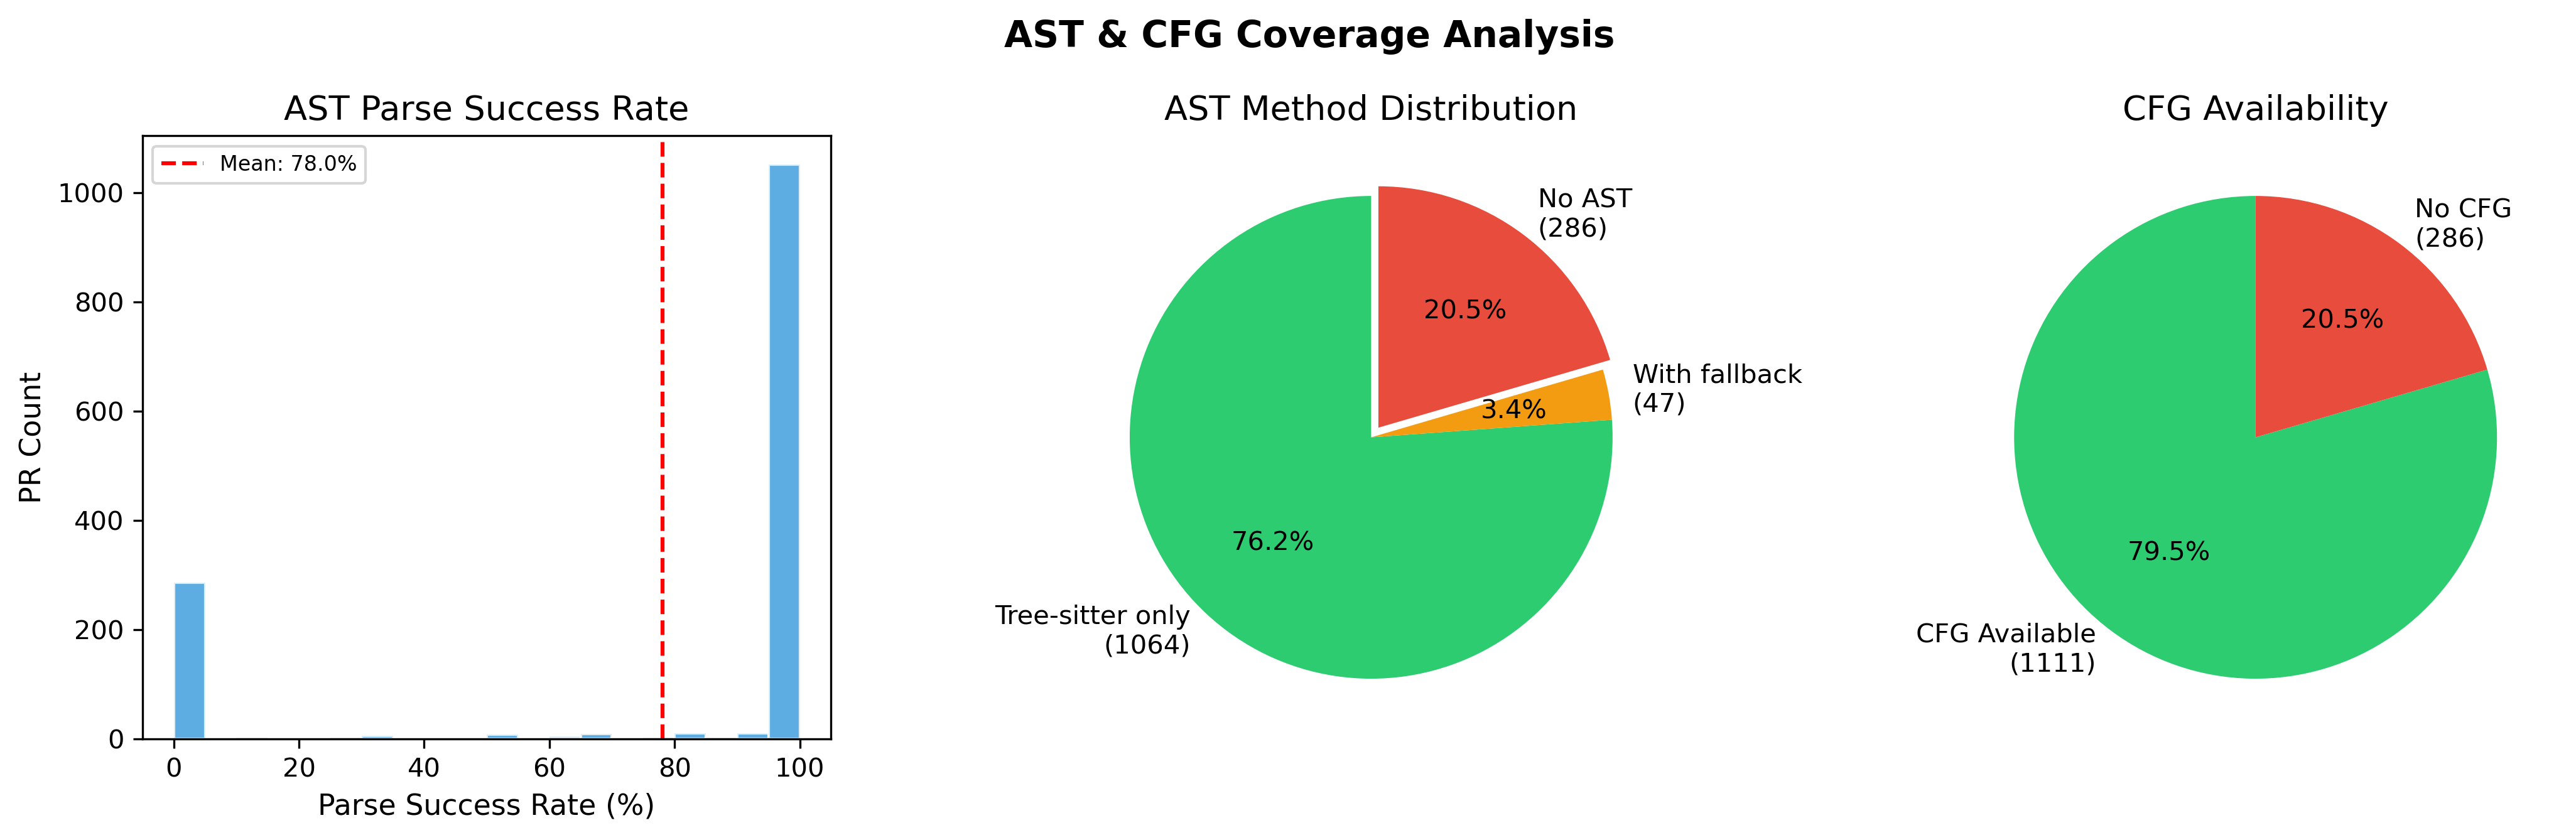
\includegraphics[width=0.95\textwidth]{../figures/03_ast_cfg_coverage.png}
\caption{AST 解析方法分布（左中）与 CFG 可用性（右）}
\end{figure}

\begin{itemize}
    \item tree-sitter 成功应用于 6 种语言（.py/.go/.js/.jsx/.ts/.tsx）；
    \item 77.7\% 的 PR 完全使用 tree-sitter，仅 3.4\% 需要 lexical fallback；
    \item 20.5\% 的 PR 无代码文件可解析（仅改文档/配置），这些样本仍保留在数据集中，AST 特征填 0 并标记；
    \item CFG 可用率 79.5\%，平均圈复杂度 67.8，与 PR 修改规模高度正相关。
\end{itemize}

\subsection*{3.3 特征工程结果}

最终主实验特征矩阵为 1397 行 $\times$ 61 列（含 59 个特征 + 2 个缺失标记）。特征间存在合理相关性：code\_churn 与 total\_additions/total\_deletions 高度正相关（r > 0.9，符合预期），AST 节点数与 CFG 节点数正相关（r $\approx$ 0.85），文本长度特征之间存在中等相关性。

\subsection*{3.4 模型实验结果}

\subsubsection*{3.4.1 主实验结果}

\begin{table}[ht]
\centering
\caption{主实验：测试集指标（无审查过程特征）}
\begin{tabular}{|l|c|c|c|c|c|}
\hline
\textbf{模型} & \textbf{Accuracy} & \textbf{Precision} & \textbf{Recall} & \textbf{F1} & \textbf{ROC-AUC} \\
\hline
Dummy (most\_frequent) & 0.6429 & -- & -- & 0.7826 & 0.5000 \\
\hline
Logistic Regression & 0.7000 & 0.7391 & 0.7556 & 0.7605 & 0.7457 \\
\hline
SVM & 0.7238 & 0.8031 & 0.7556 & 0.7786 & 0.7788 \\
\hline
\textbf{Random Forest} & \textbf{0.7429} & \textbf{0.7455} & \textbf{0.9111} & \textbf{0.8200} & \textbf{0.8062} \\
\hline
\end{tabular}
\end{table}

\textbf{分析：}
\begin{itemize}
    \item 所有训练模型均明显超过 Dummy baseline（Acc 0.64），验证了特征的有效性；
    \item Random Forest 优于 SVM（Acc 0.7429 vs 0.7238，AUC 0.8062 vs 0.7788），符合 RF 对非线性特征和异常值更鲁棒的预期；
    \item RF 的 Recall（0.9111）远高于 SVM（0.7556），说明 RF 更擅长识别会合并的 PR。RF 的 Precision（0.7455）低于 SVM（0.8031），存在一定的假阳性；
    \item 主实验 AUC 0.8062，达到了计划书预期的 0.70--0.82 范围，合理且可信。
\end{itemize}

\subsubsection*{3.4.2 上界扩展实验结果}

\begin{table}[ht]
\centering
\caption{上界实验：测试集指标（含审查过程特征）}
\begin{tabular}{|l|c|c|c|c|c|}
\hline
\textbf{模型} & \textbf{Accuracy} & \textbf{Precision} & \textbf{Recall} & \textbf{F1} & \textbf{ROC-AUC} \\
\hline
SVM & 0.8619 & 0.8786 & 0.9111 & 0.8945 & 0.9111 \\
\hline
\textbf{Random Forest} & \textbf{0.9000} & \textbf{0.9318} & \textbf{0.9111} & \textbf{0.9213} & \textbf{0.9546} \\
\hline
\end{tabular}
\end{table}

上界实验指标显著高于主实验（RF Acc +0.157, AUC +0.148），这直观地验证了审查过程特征（review\_decision、num\_reviewers、num\_review\_comments 等）携带大量后验信息。这一差距清楚地说明了为什么主实验必须严格排除这些字段——如果不加控制，模型将学到"被 approve 的 PR 更可能合并"这种后验规律，虽然在测试集上分数很高，但实际应用时（PR 刚提交、审查尚未完成）完全不可用。

\clearpage

\subsection*{3.5 特征重要性分析}

\begin{figure}[ht]
\centering
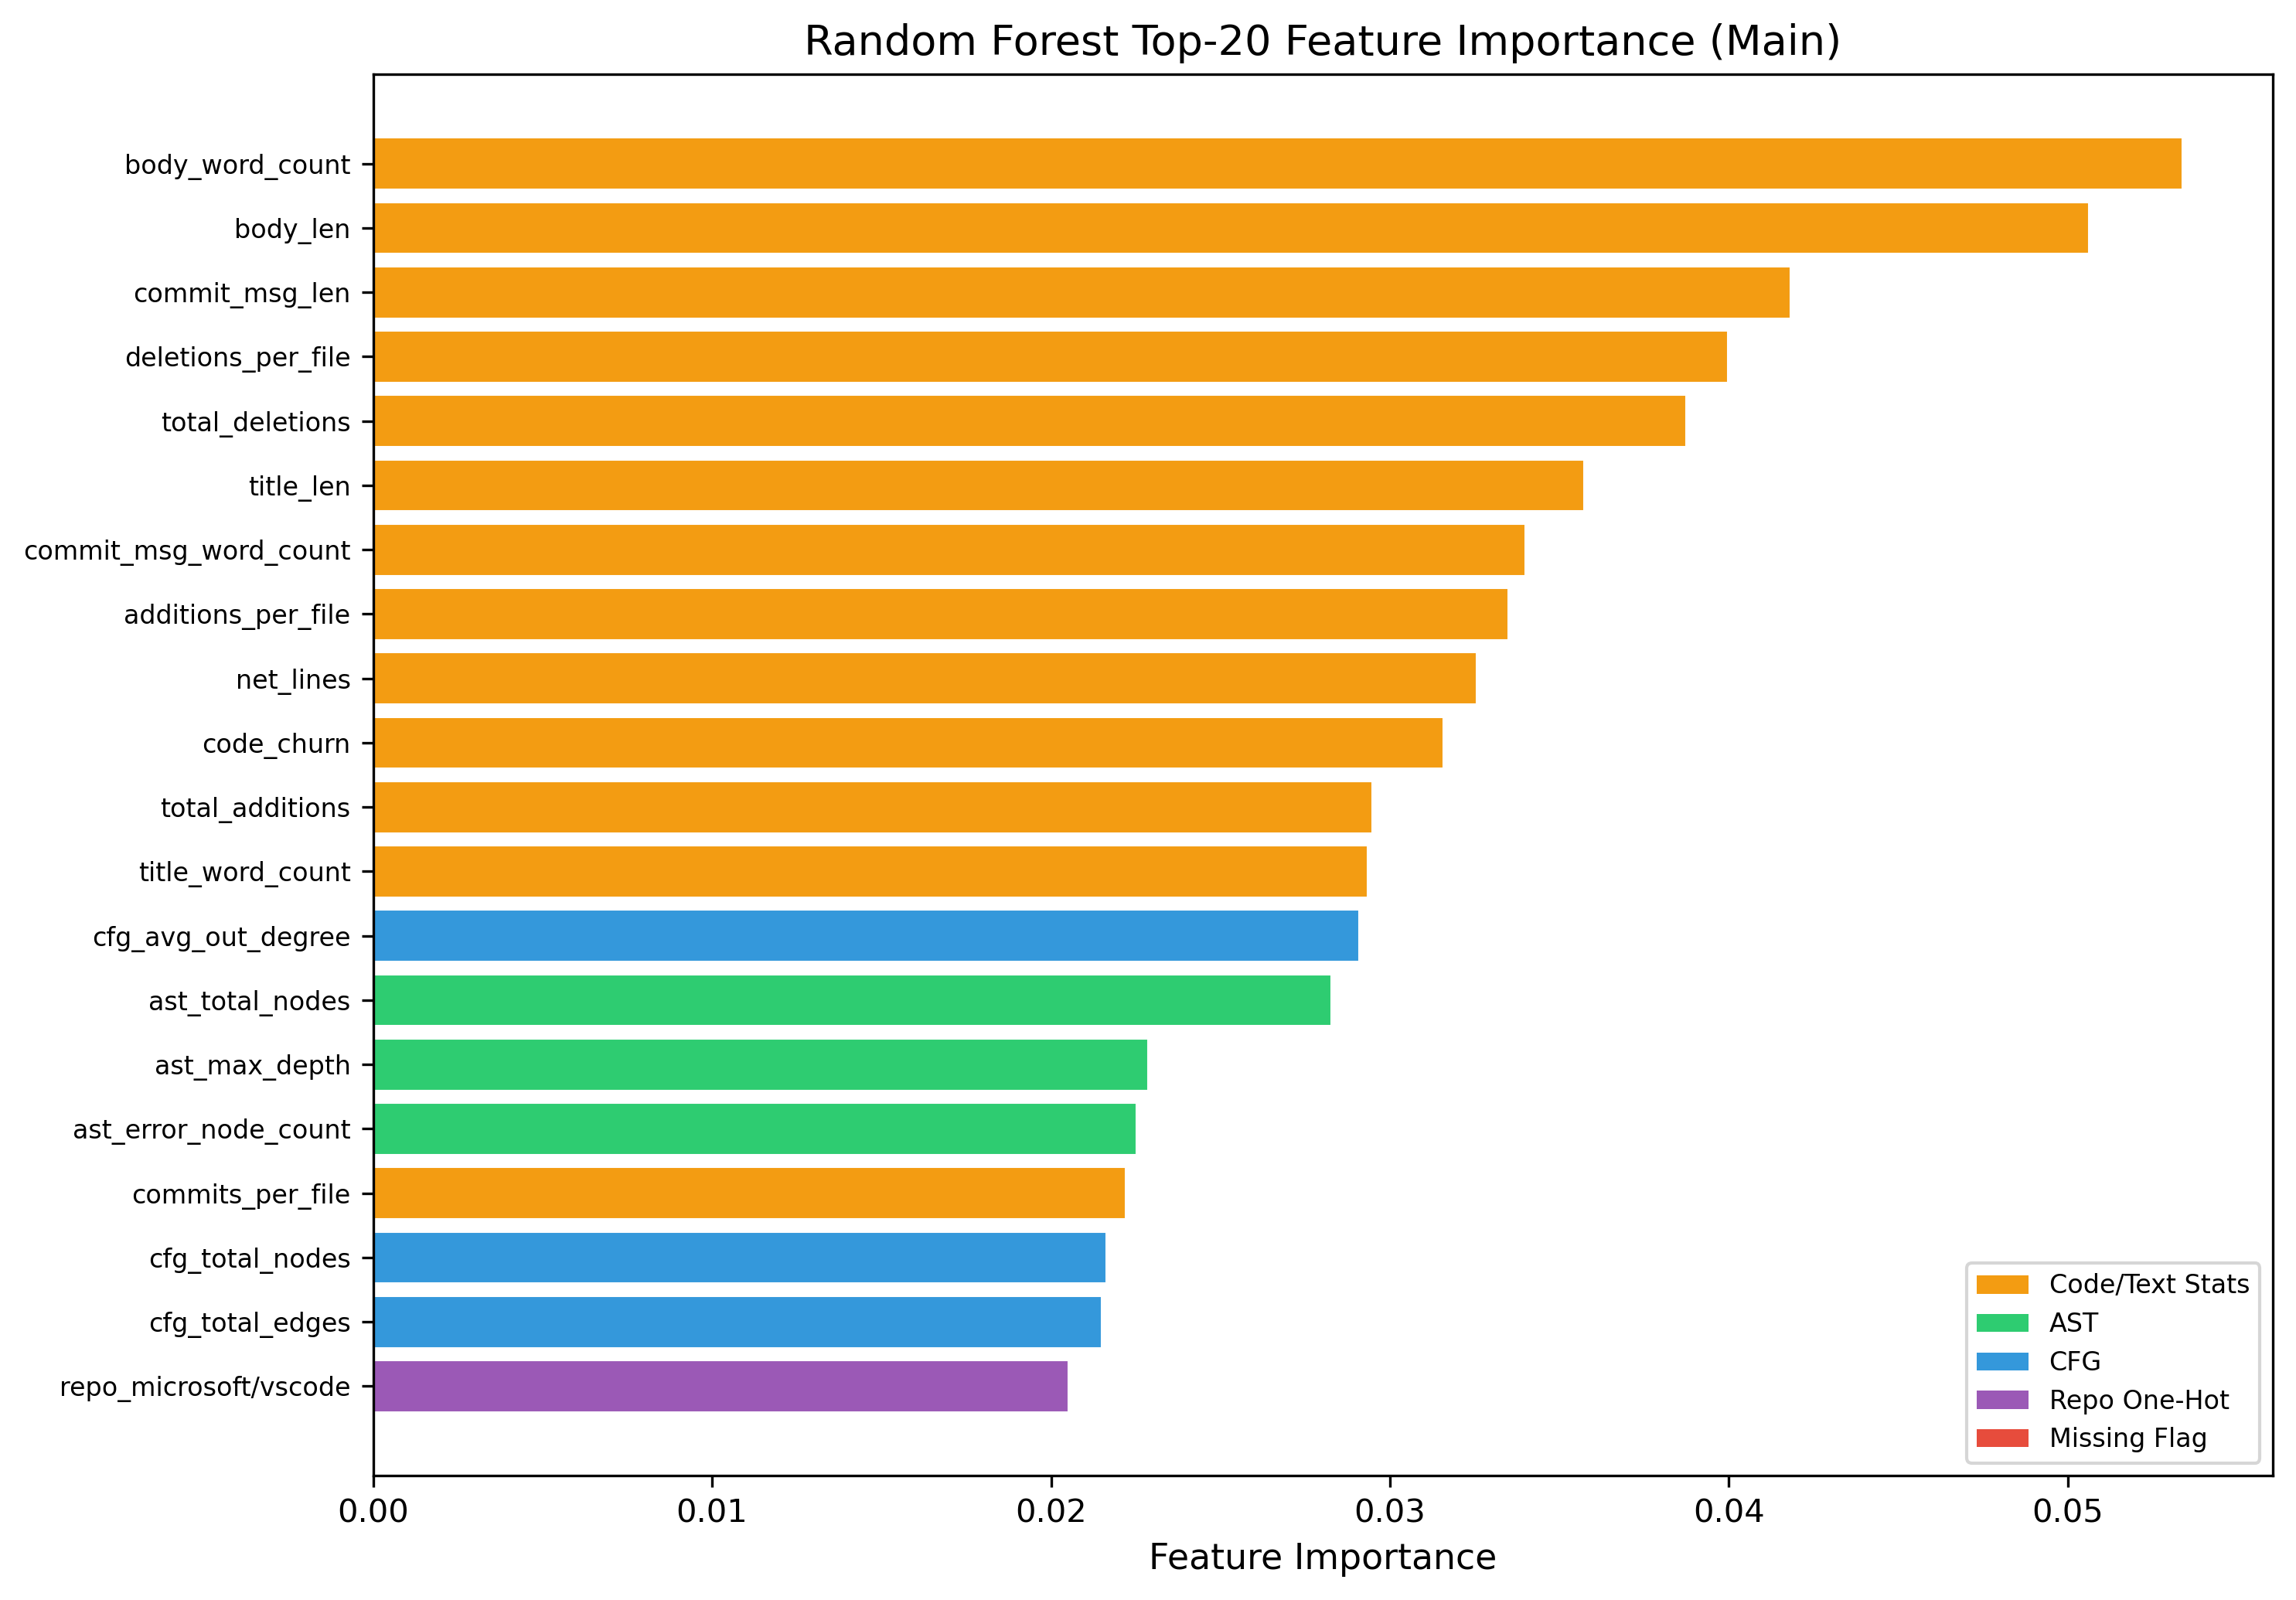
\includegraphics[width=\textwidth]{../figures/08_feature_importance.png}
\caption{Random Forest Top-20 特征重要性（主实验）}
\end{figure}

Top-5 特征：
\begin{enumerate}
    \item \textbf{body\_word\_count}（0.0534）—— PR 描述的详细程度是最重要的预测因子；
    \item \textbf{body\_len}（0.0506）—— 描述越长，信息量越大，合并概率越高；
    \item \textbf{commit\_msg\_len}（0.0418）—— Commit Message 的详细程度；
    \item \textbf{deletions\_per\_file}（0.0400）—— 每文件删除行数，反映了重构程度；
    \item \textbf{total\_deletions}（0.0387）—— 总删除行数。
\end{enumerate}

特征重要性呈现清晰的层次结构：
\begin{itemize}
    \item \textbf{文本特征（4/5）}占据主导地位，说明在 PR 提交时，描述和 Message 的质量是决定是否合并的最强信号；
    \item \textbf{代码修改规模特征}紧随其后（additions\_per\_file, code\_churn, total\_additions），修改量小且聚焦的 PR 更易合并；
    \item \textbf{CFG 特征}（cfg\_avg\_out\_degree, cfg\_total\_nodes）排名 13--19，结构特征有贡献但非主导；
    \item \textbf{AST 特征}（ast\_total\_nodes, ast\_max\_depth）排名 14--16；
    \item \textbf{仓库 One-Hot}中 microsoft/vscode 排名第 20，说明合并率较高的仓库本身带有一定预测信息，但影响力有限。
\end{itemize}

\subsection*{3.6 消融实验结果}

\begin{figure}[ht]
\centering
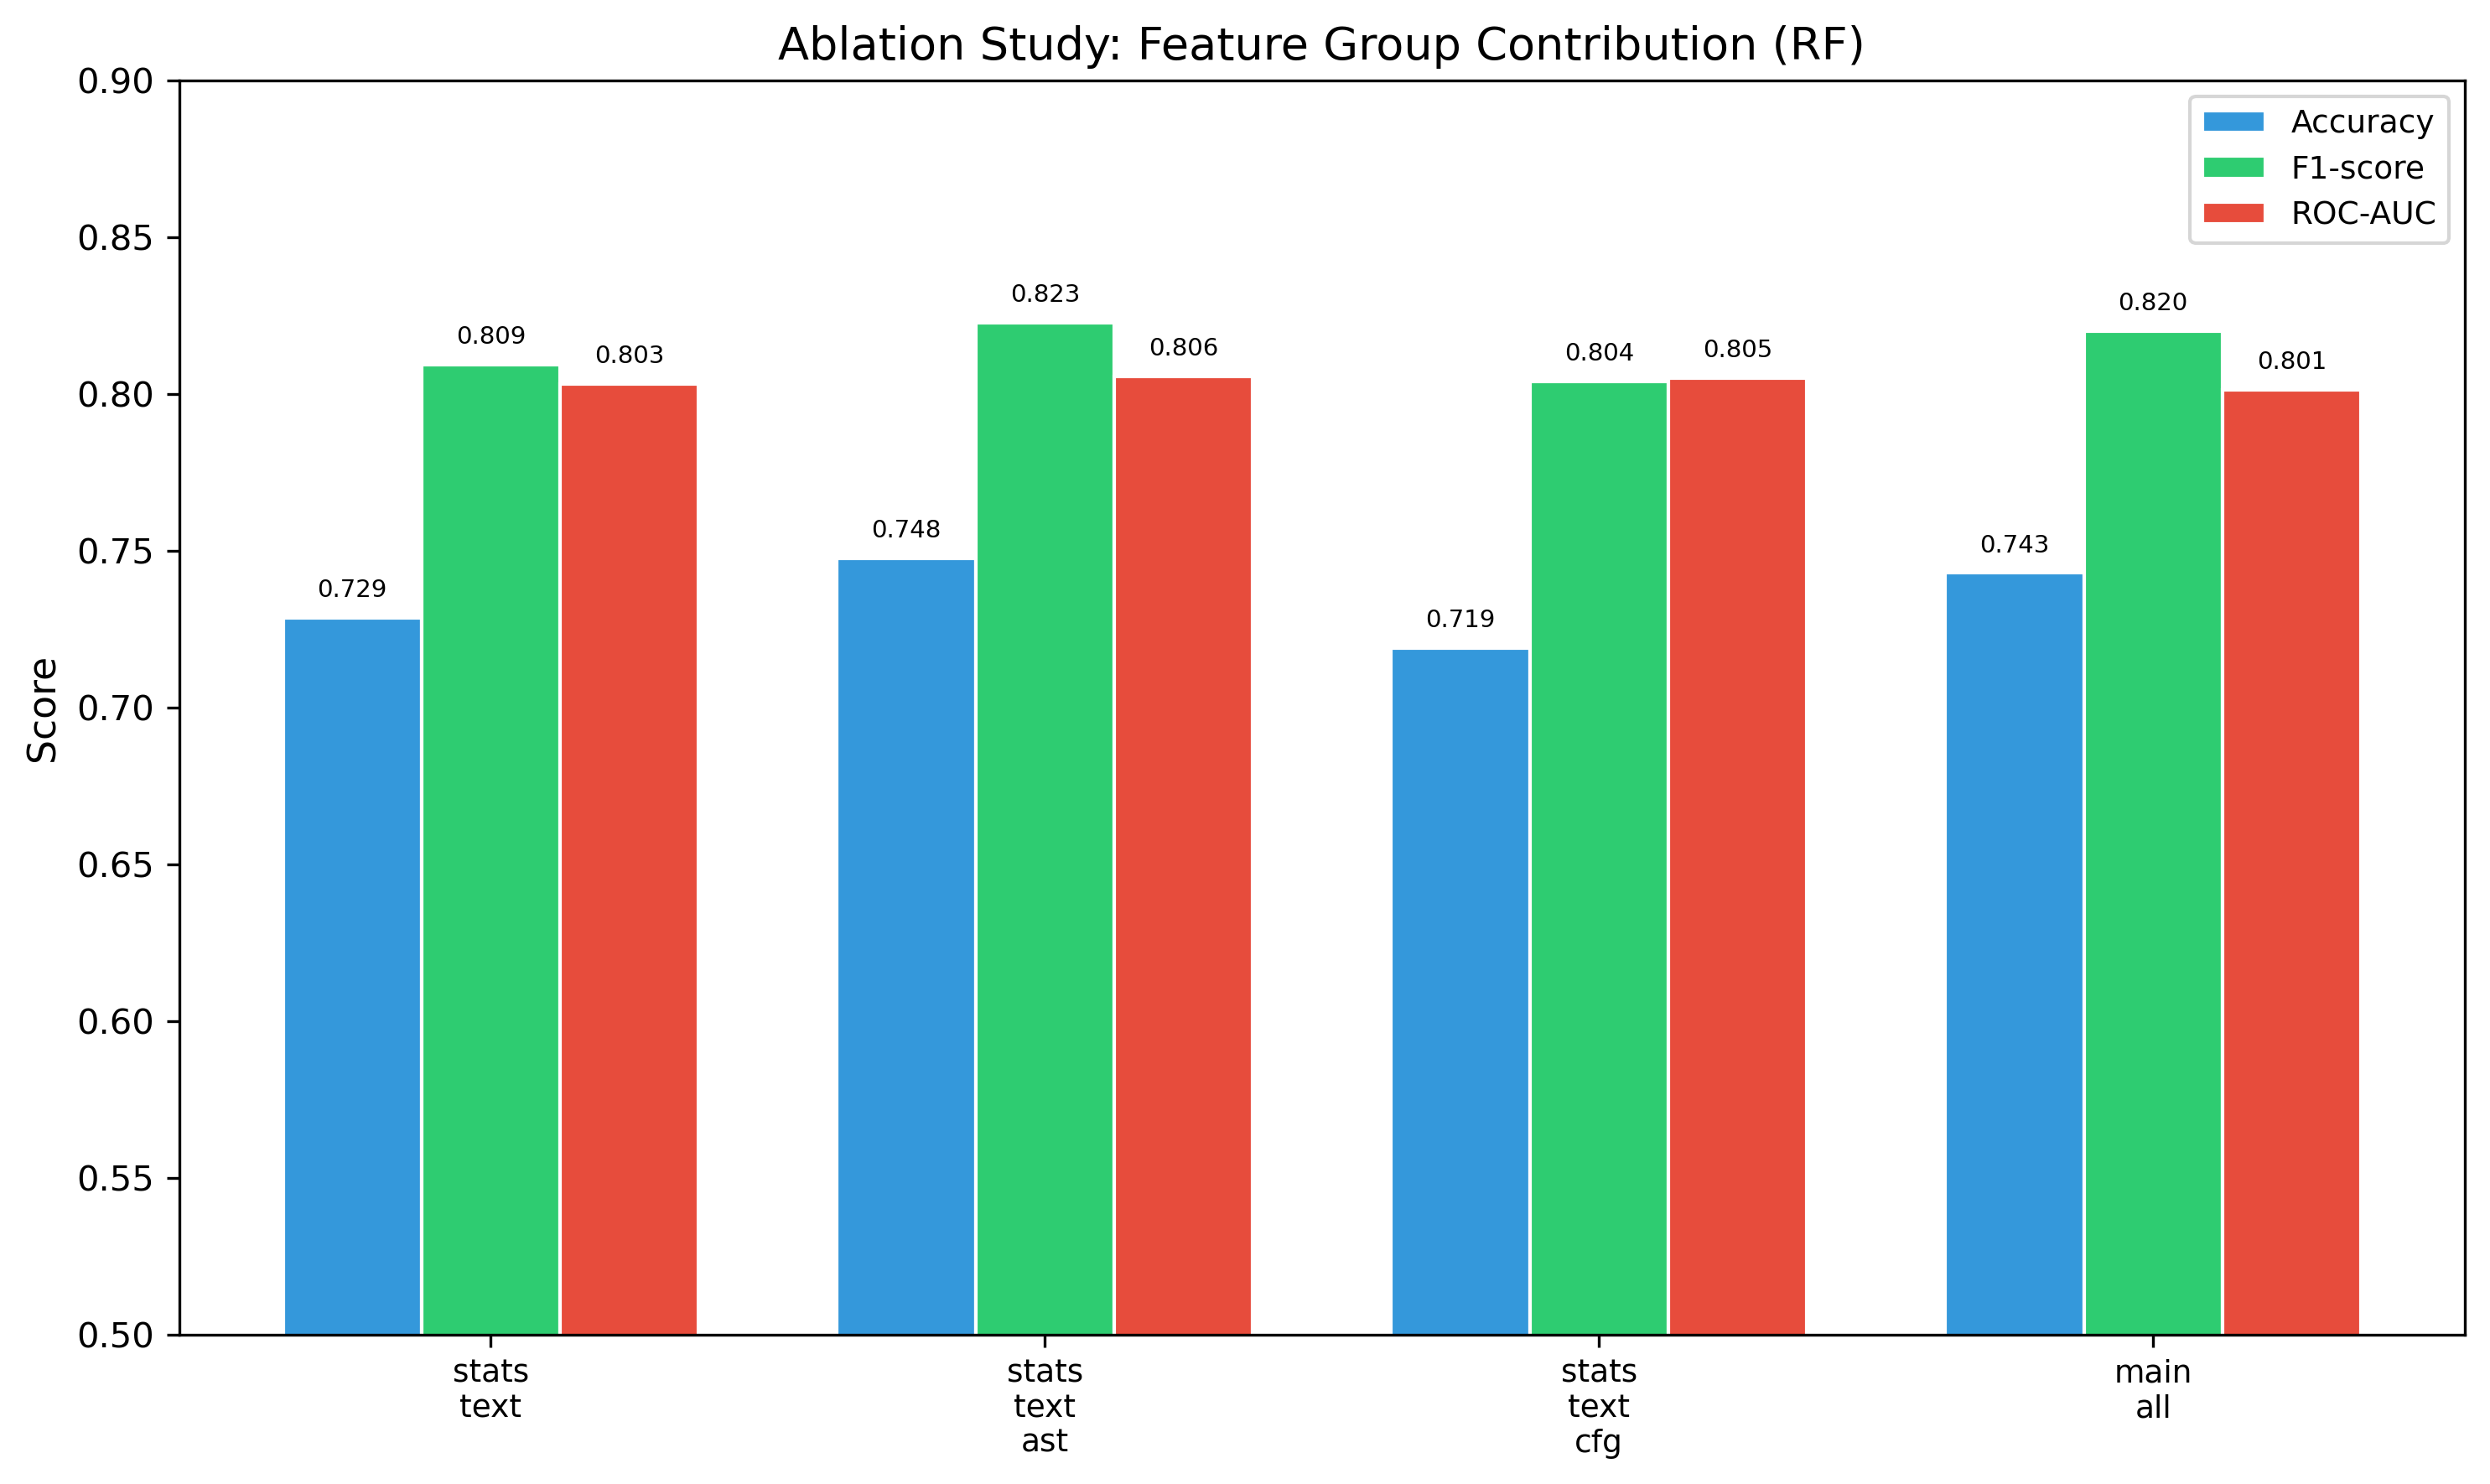
\includegraphics[width=\textwidth]{../figures/09_ablation_comparison.png}
\caption{特征组消融实验对比}
\end{figure}

\begin{table}[ht]
\centering
\caption{消融实验详细指标}
\begin{tabular}{|l|c|c|c|c|}
\hline
\textbf{特征组} & \textbf{特征数} & \textbf{Accuracy} & \textbf{F1} & \textbf{ROC-AUC} \\
\hline
stats\_text & 36 & 0.7286 & 0.8094 & 0.8033 \\
\hline
stats\_text\_ast & 50 & \textbf{0.7476} & \textbf{0.8227} & \textbf{0.8057} \\
\hline
stats\_text\_cfg & 47 & 0.7190 & 0.8040 & 0.8051 \\
\hline
main\_all & 61 & 0.7429 & 0.8200 & 0.8013 \\
\hline
\end{tabular}
\end{table}

\textbf{分析：}
\begin{itemize}
    \item 加入 AST 特征后，Acc 从 0.7286 提升至 0.7476（+1.9\%），F1 从 0.8094 提升至 0.8227，说明 AST 结构信息提供了有效的增量预测能力；
    \item 单独加入 CFG 特征时 Acc 下降至 0.7190（-0.96\%），可能是 CFG 特征含有一定噪声，但 AUC 仍有轻微提升（0.8033 $\to$ 0.8051）；
    \item main\_all 同时加入 AST+CFG 达到了最高的 F1（0.8200），但 AUC 与 stats\_text 基本持平（0.8013 vs 0.8033），表明 AST/CFG 特征的边际贡献有限；
    \item 这一发现本身具有研究价值：对于 patch 级别的代码片段，传统结构特征的表达能力确实不如完整文件级别的 AST/CFG。这为后续使用 Code2Vec、CodeBERT 等深度学习方法（能自动学习代码表示）提供了动机。
\end{itemize}

\subsection*{3.7 模型性能对比}

\begin{figure}[ht]
\centering
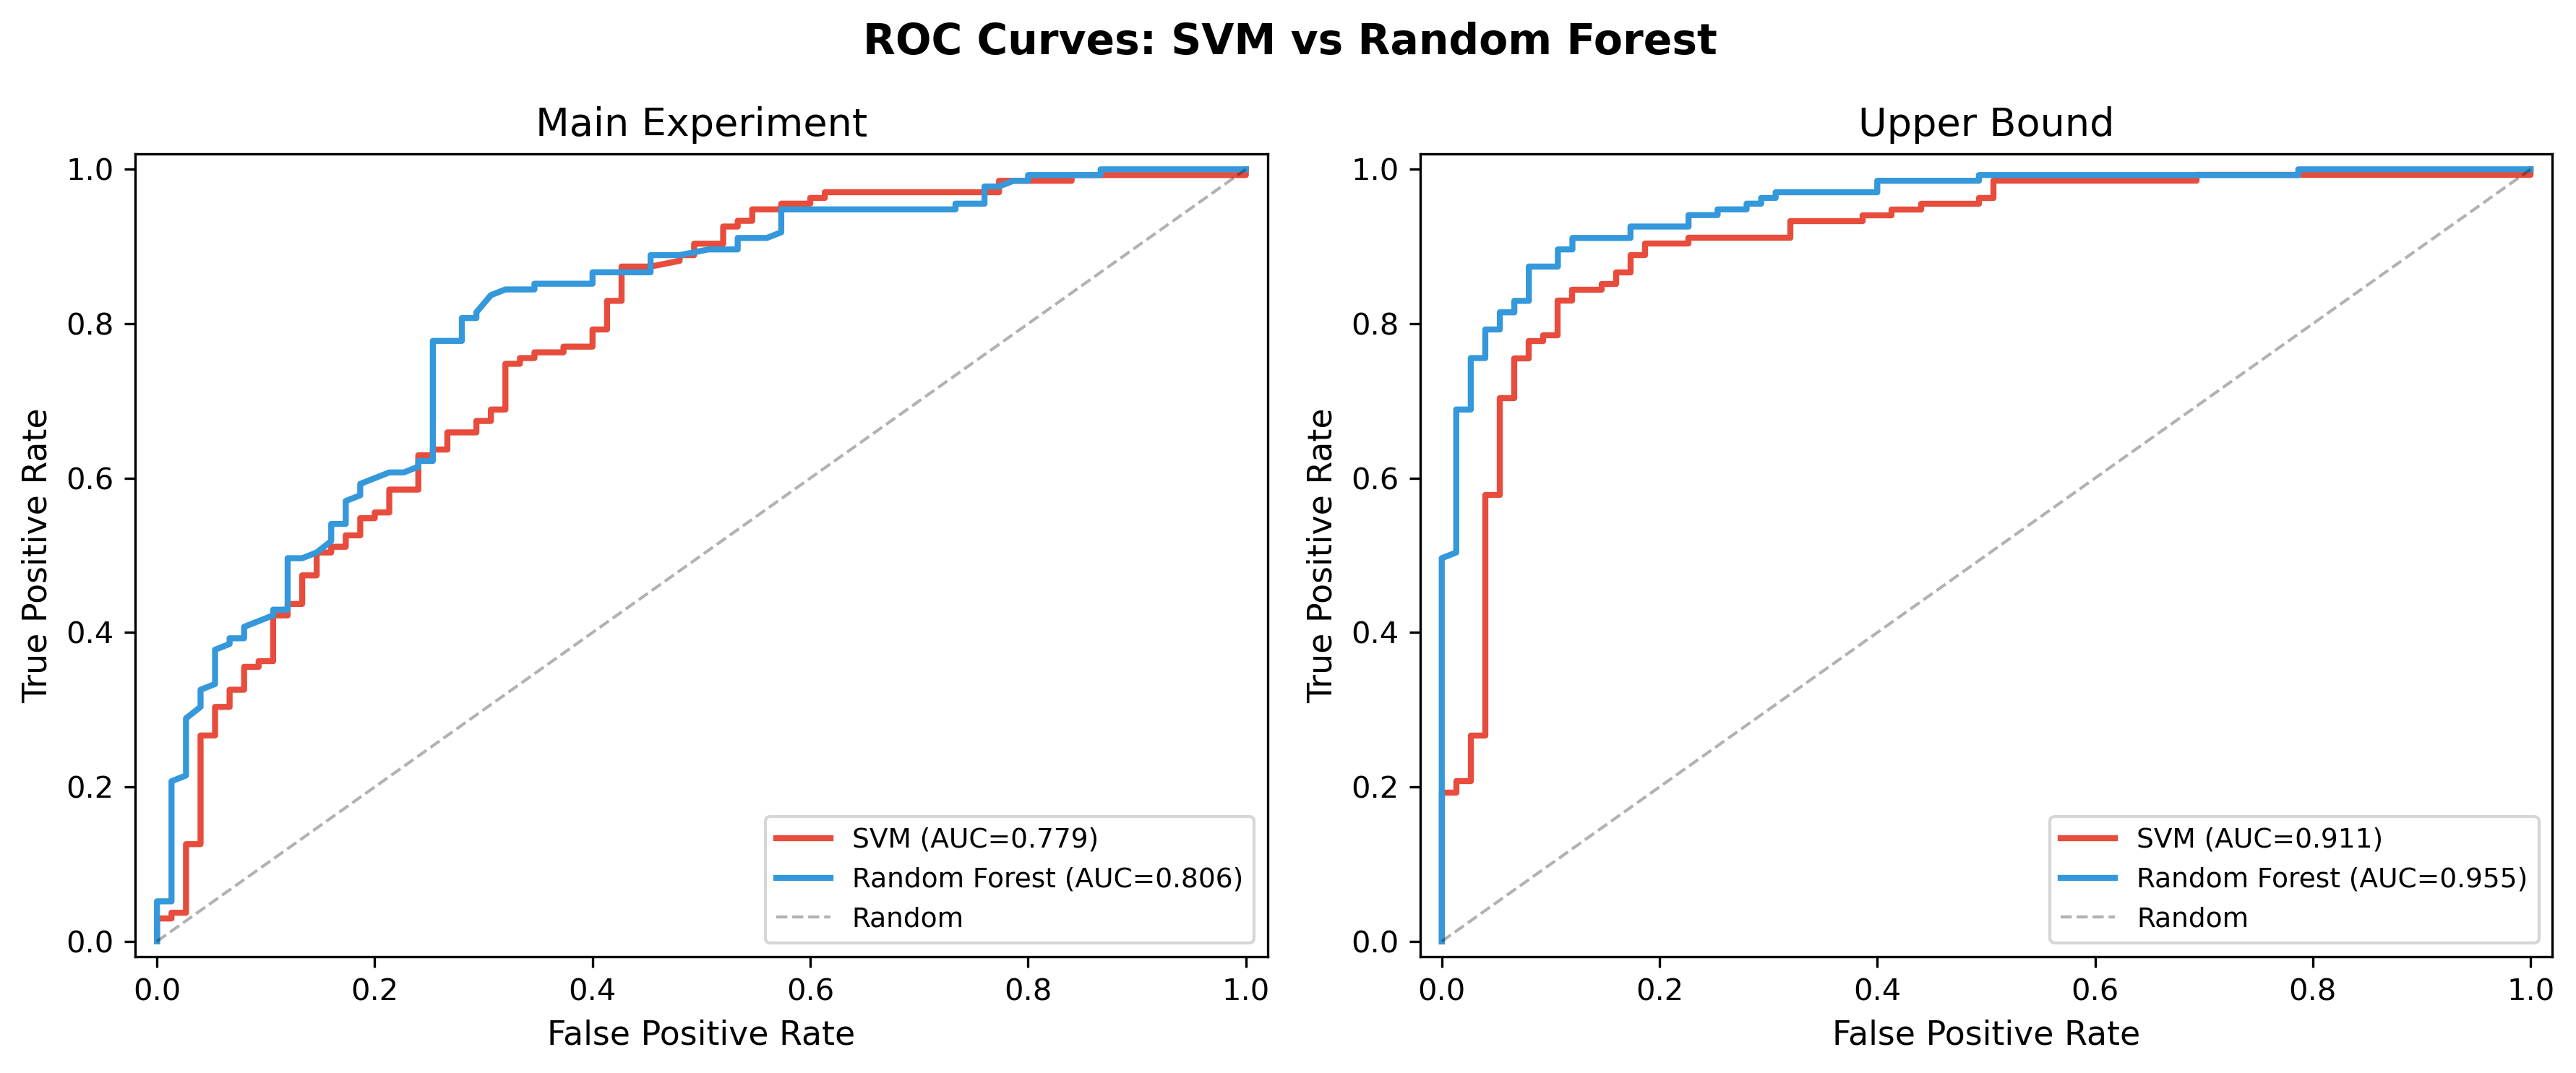
\includegraphics[width=0.75\textwidth]{../figures/05_roc_curve_main.png}
\caption{主实验（左）与上界实验（右）ROC 曲线对比}
\end{figure}

\subsection*{3.8 分仓库性能}

\begin{table}[ht]
\centering
\caption{Random Forest 主实验分仓库性能}
\begin{tabular}{|l|c|c|c|c|}
\hline
\textbf{仓库} & \textbf{样本数} & \textbf{Accuracy} & \textbf{F1} & \textbf{ROC-AUC} \\
\hline
facebook/react & 45 & 0.7556 & 0.7843 & 0.8953 \\
\hline
huggingface/transformers & 45 & 0.7556 & 0.8000 & 0.8170 \\
\hline
kubernetes/kubernetes & 45 & 0.5778 & 0.7164 & 0.5267 \\
\hline
microsoft/vscode & 31 & 0.9032 & 0.9492 & 0.6310 \\
\hline
pandas-dev/pandas & 44 & 0.7727 & 0.8529 & 0.8119 \\
\hline
\end{tabular}
\end{table}

Kubernetes 的性能明显低于其他仓库（Acc 0.5778，AUC 0.5267）。可能原因：Kubernetes 的 PR 审查流程较为特殊（SIG 机制、多阶段审查），仅靠代码修改和文本特征难以充分建模。VSCode 的 Acc 最高（0.9032）但 AUC 偏低（0.6310），这与测试集中 VSCode 正样本占比较高（合并率 87.1\%）有关——模型倾向于预测"合并"即可获得高准确率。

\subsection*{3.9 可视化分析}

\begin{figure}[ht]
\centering
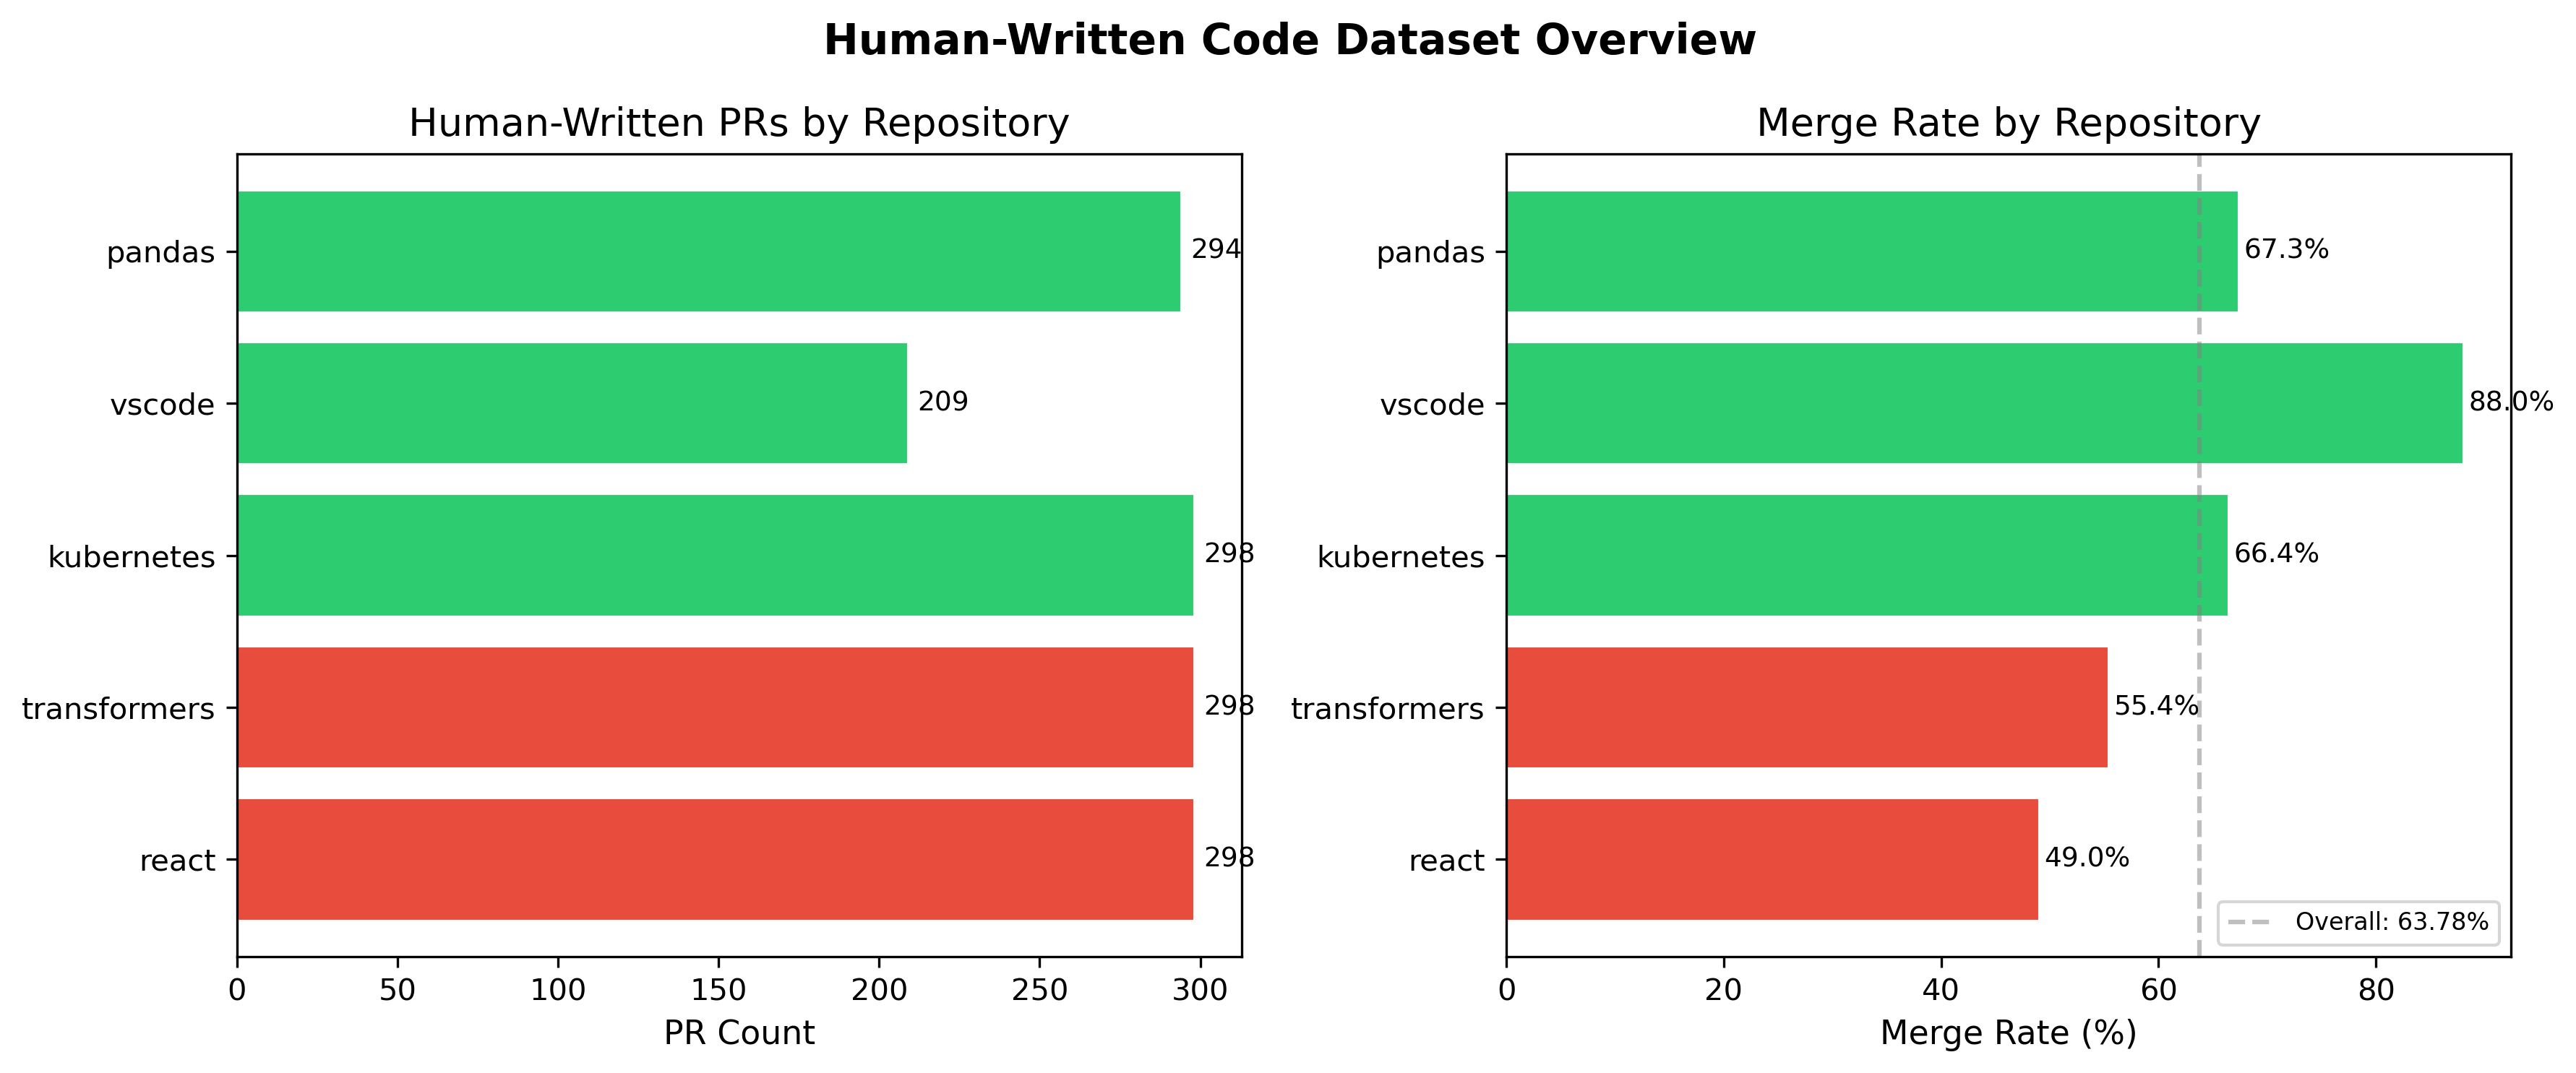
\includegraphics[width=0.9\textwidth]{../figures/01_human_dataset_distribution.png}
\caption{人类代码数据集仓库分布与合并率}
\end{figure}

\begin{figure}[ht]
\centering
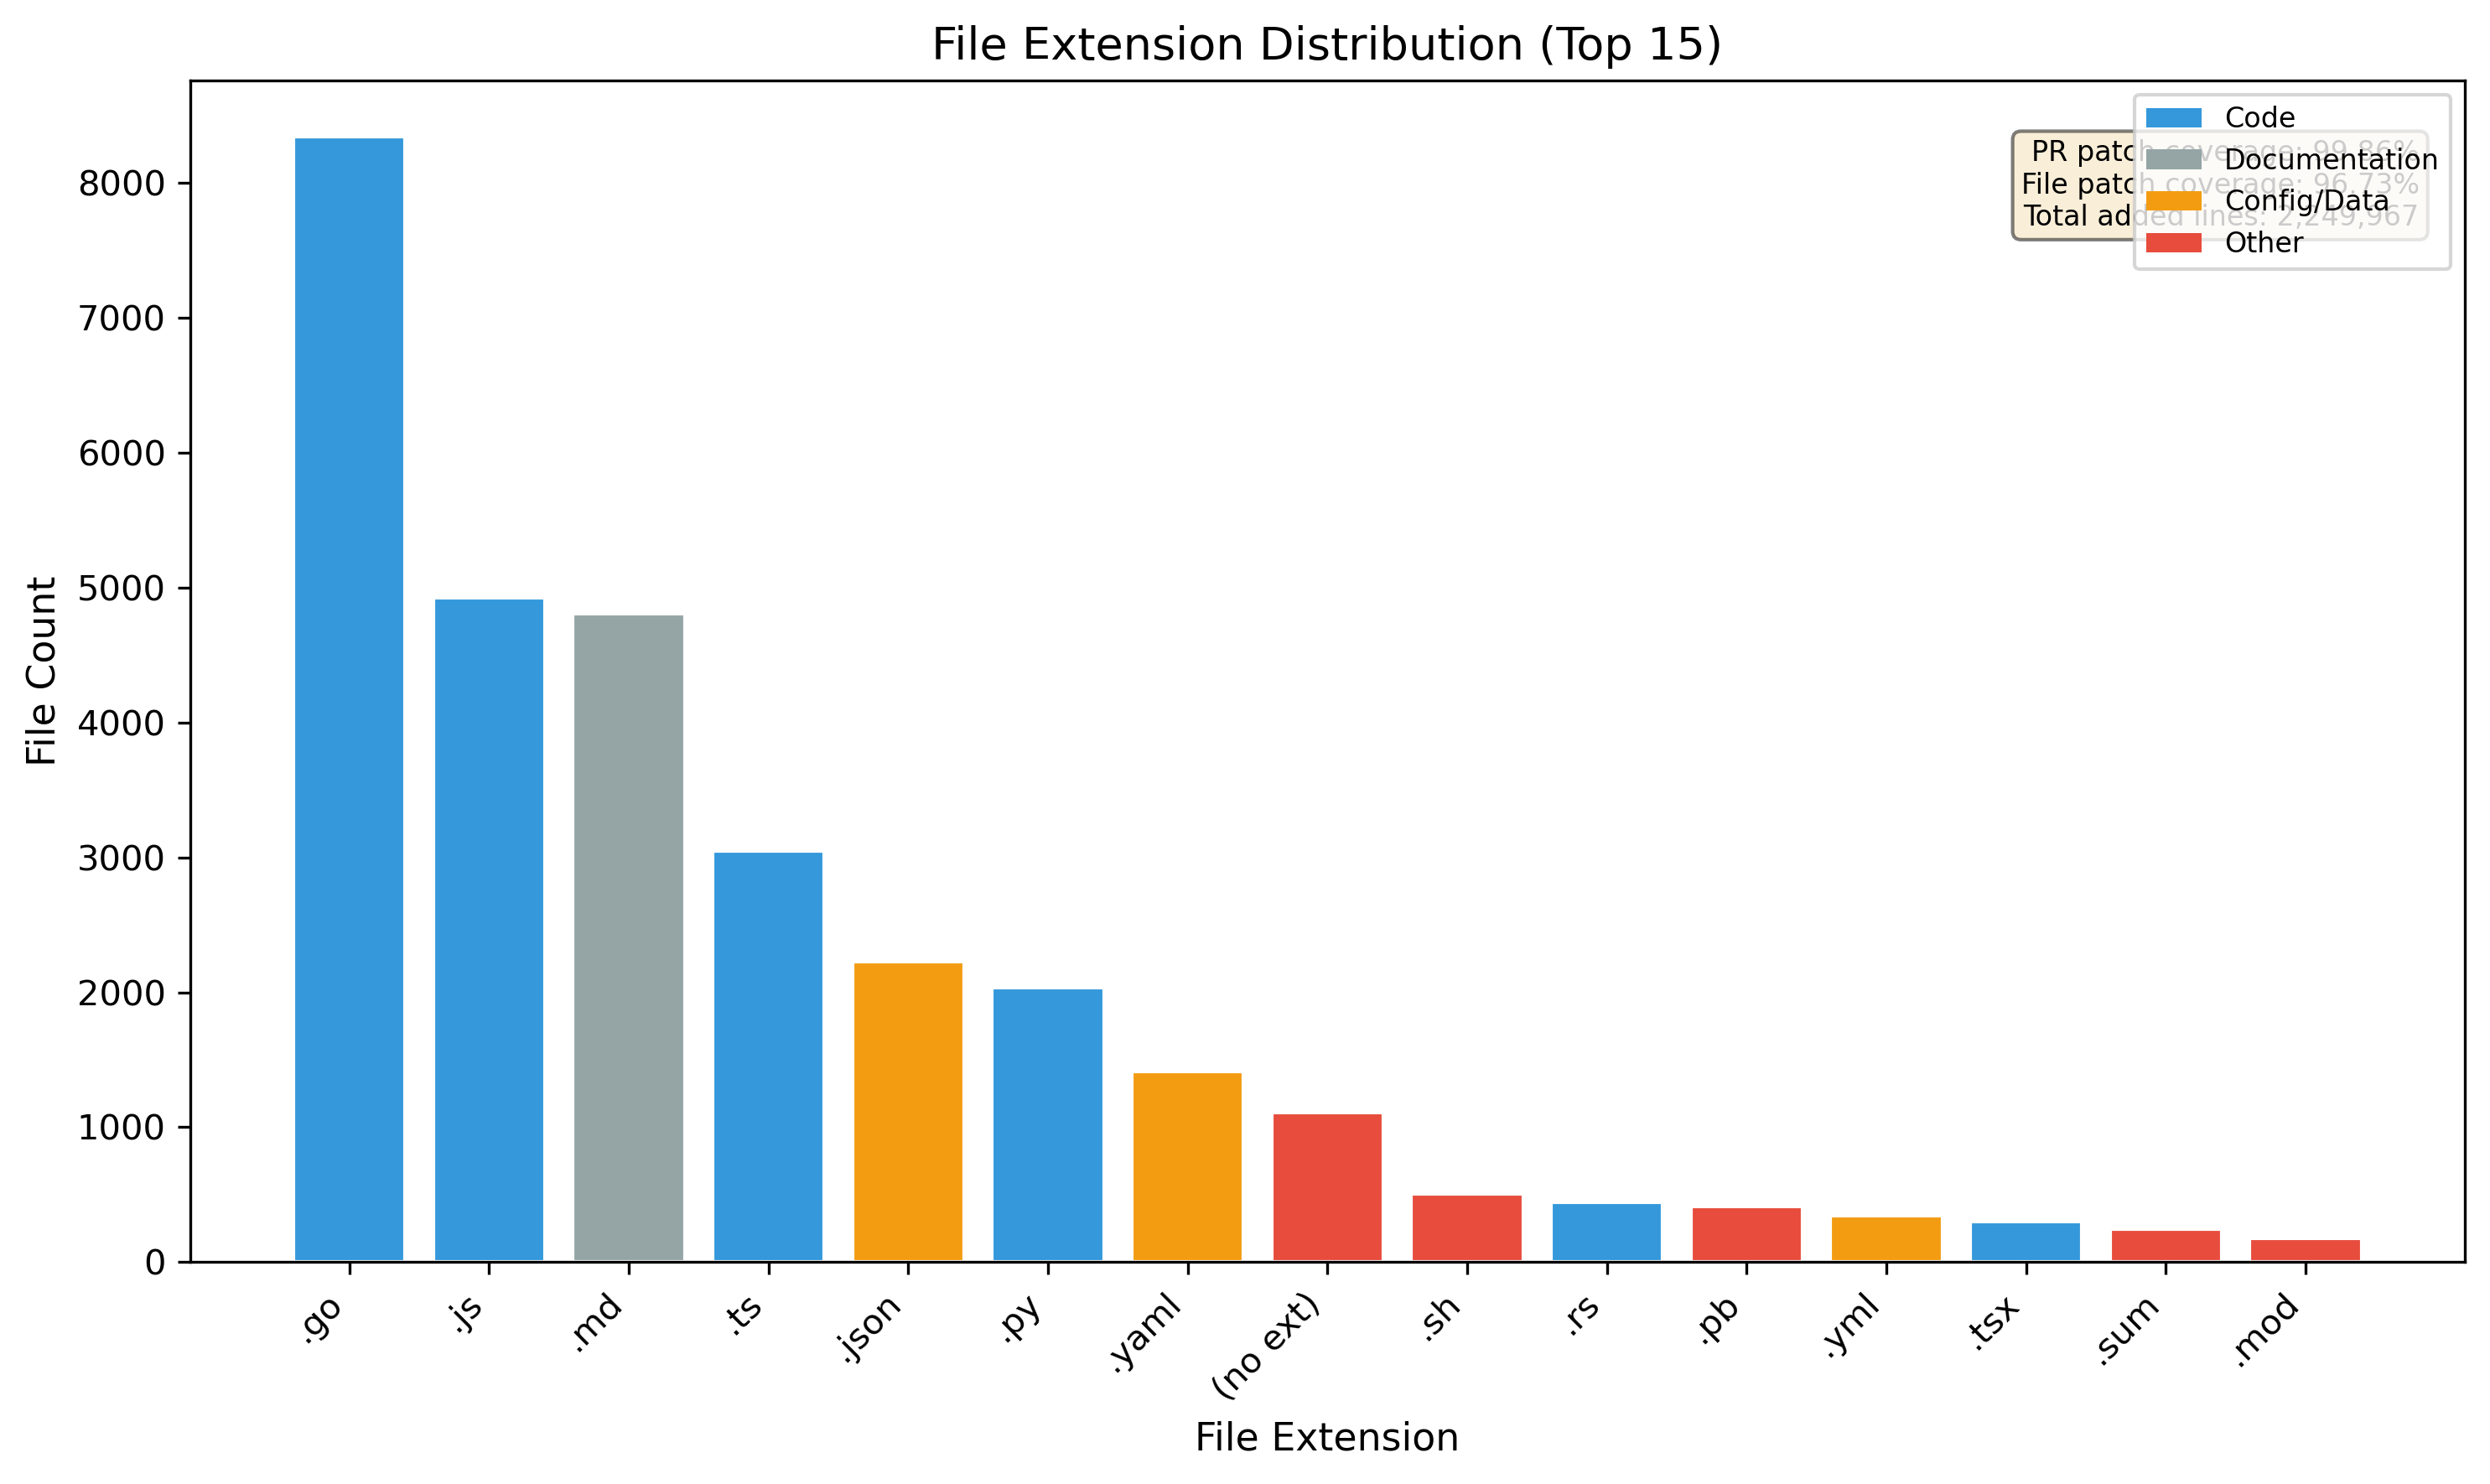
\includegraphics[width=0.9\textwidth]{../figures/02_language_patch_coverage.png}
\caption{文件扩展名分布与 Patch 覆盖率}
\end{figure}

\begin{figure}[ht]
\centering
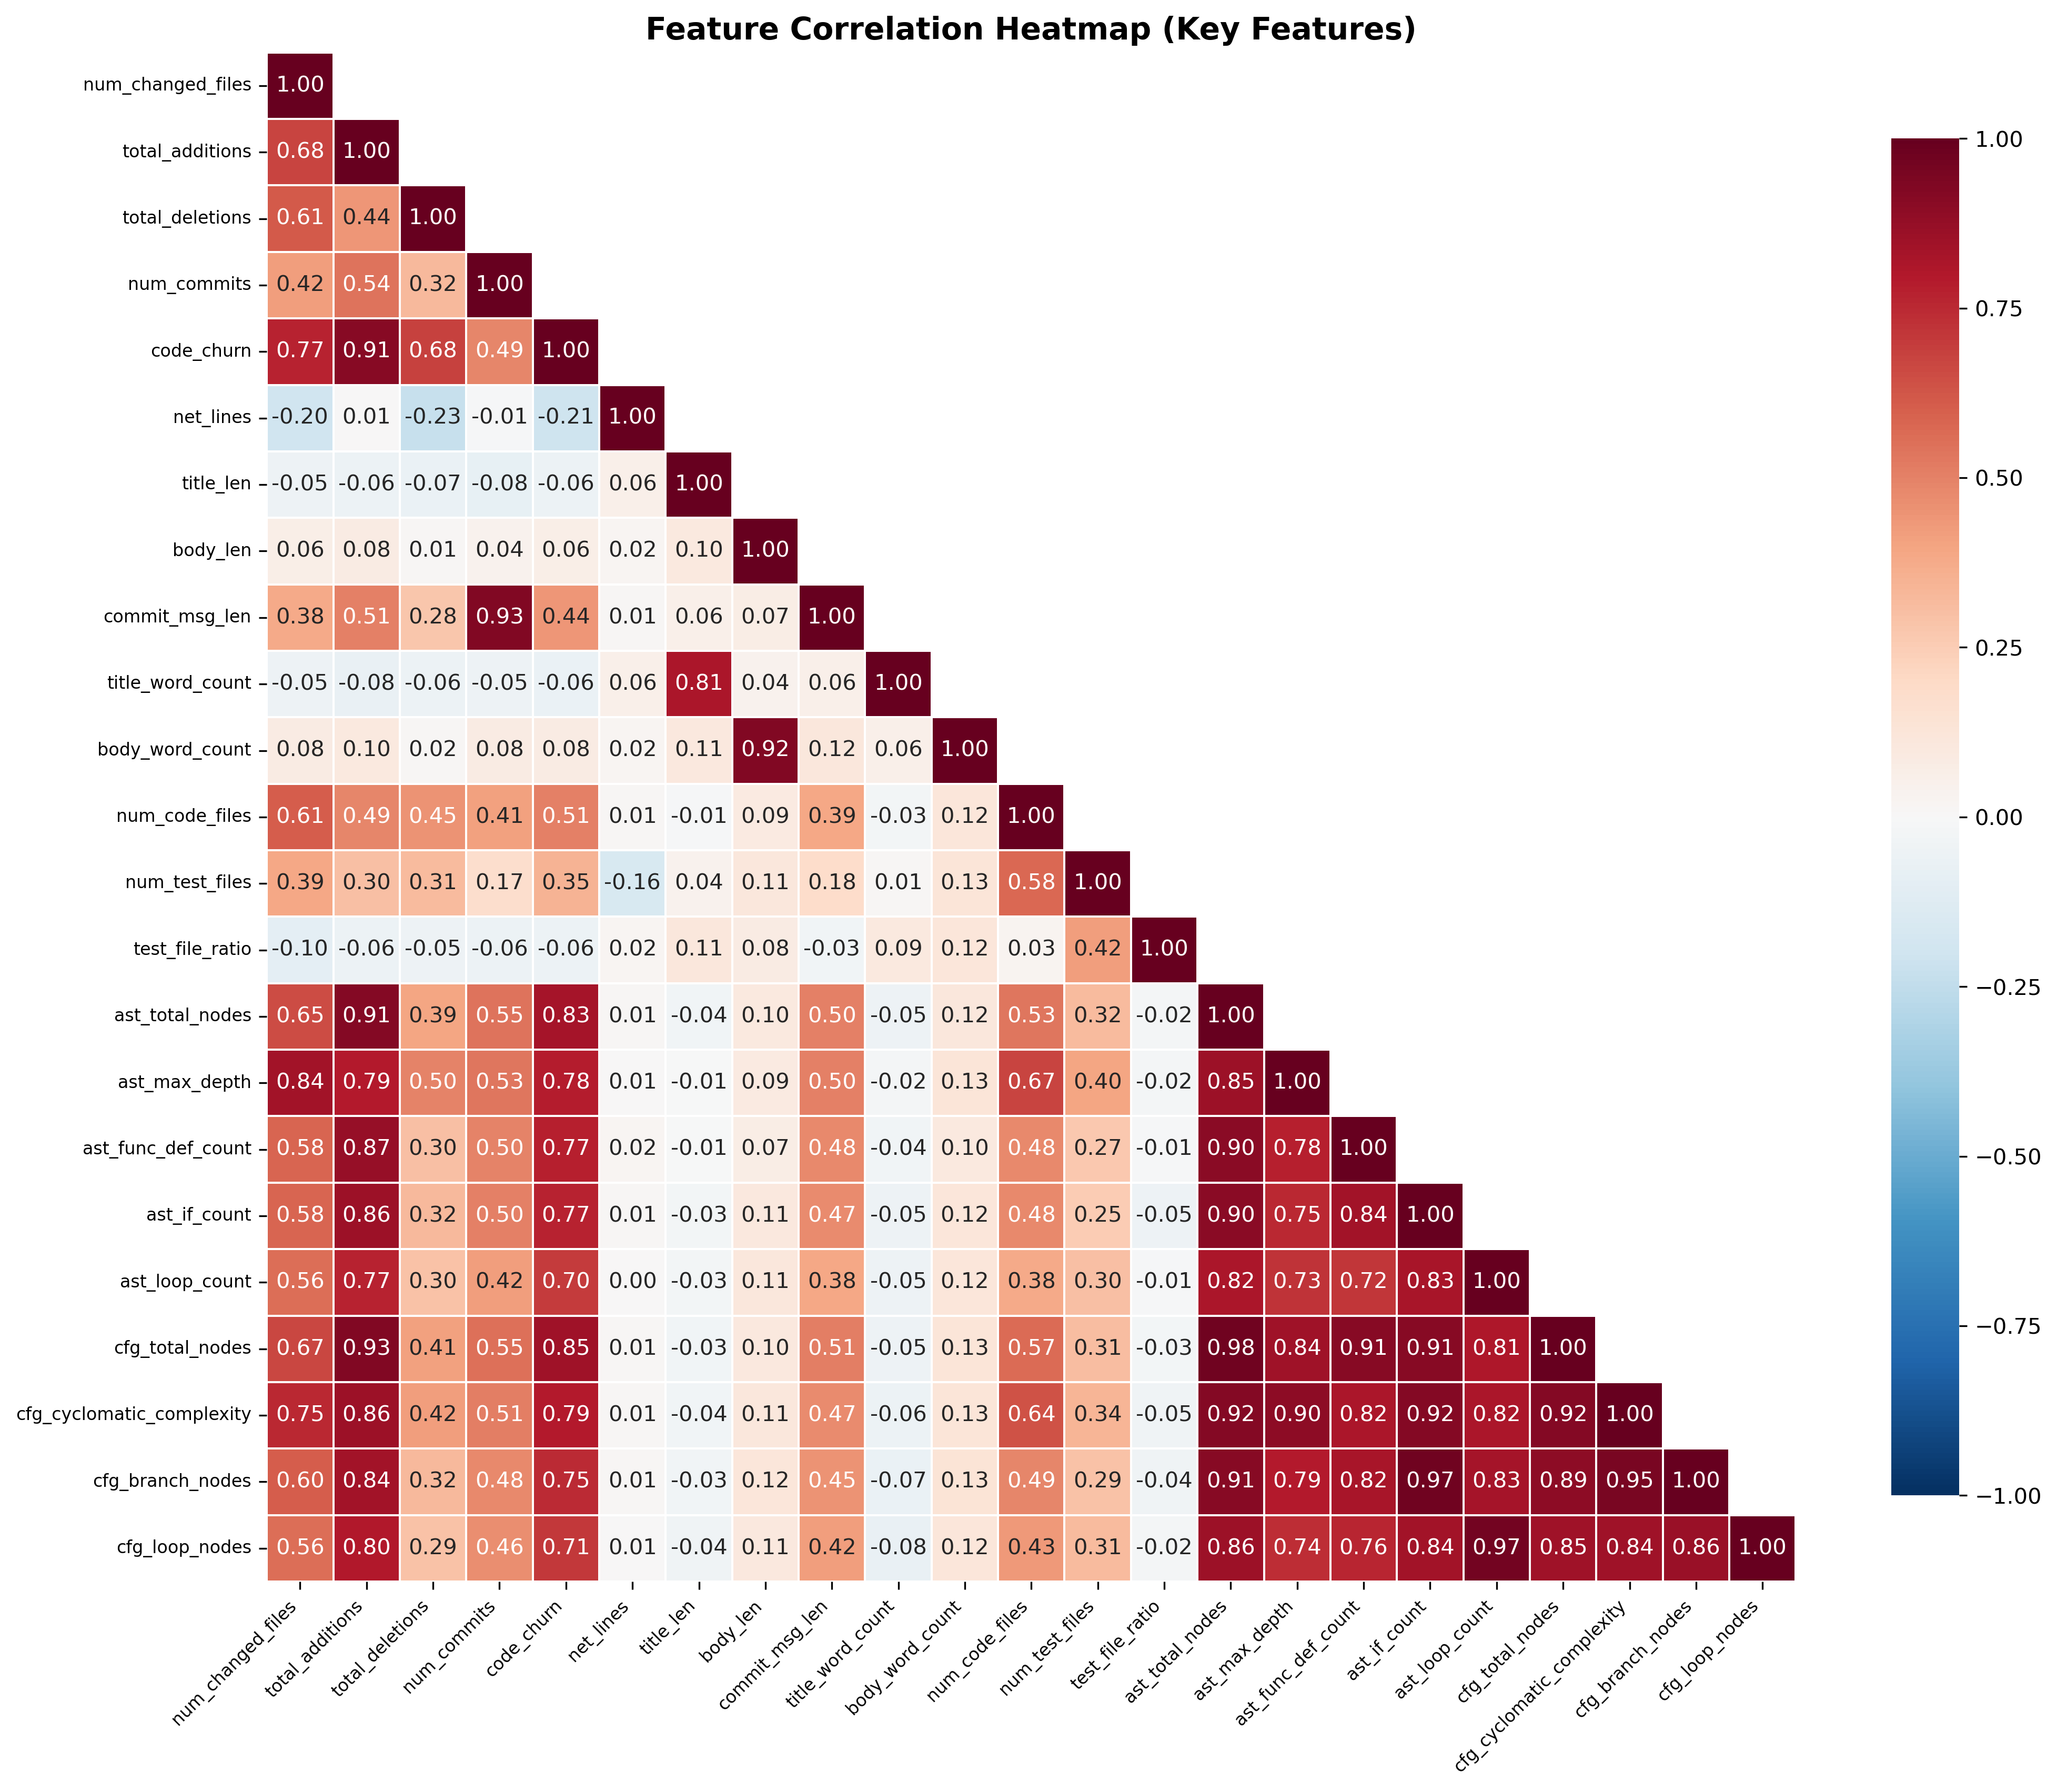
\includegraphics[width=0.9\textwidth]{../figures/04_feature_correlation_heatmap.png}
\caption{关键特征相关性热力图}
\end{figure}

\begin{figure}[ht]
\centering
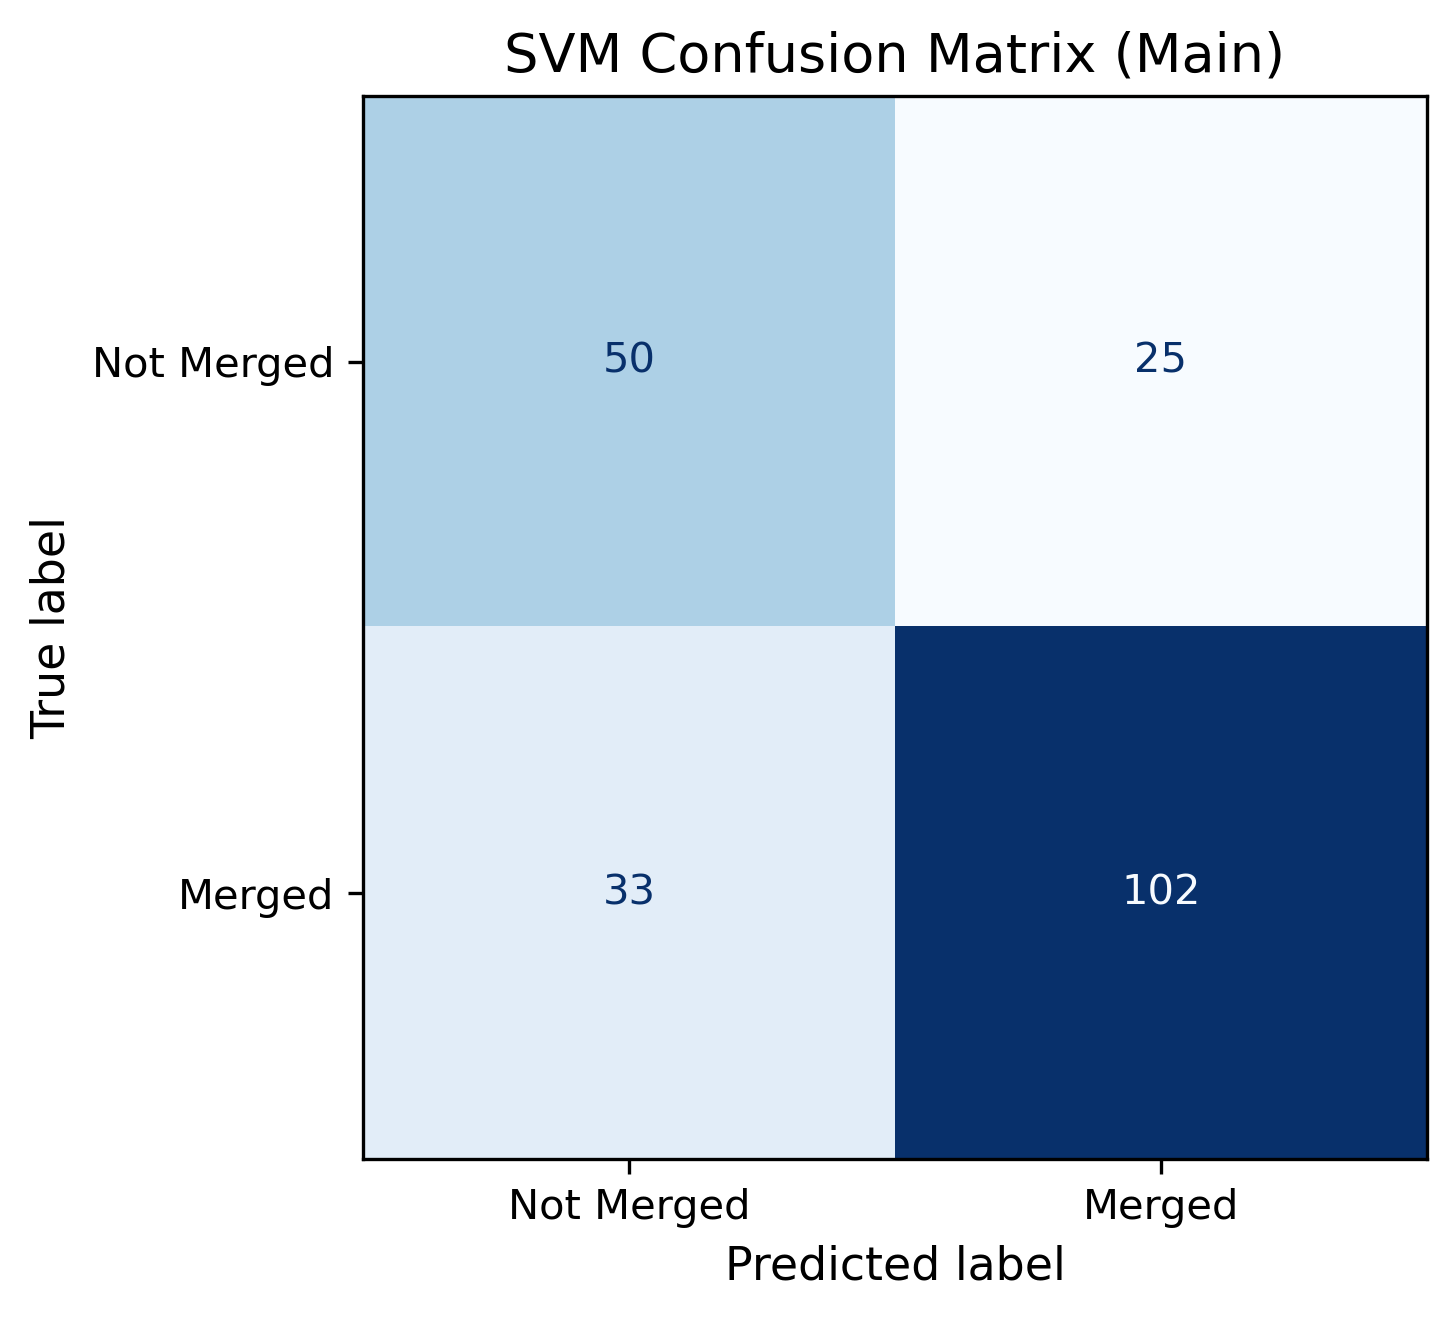
\includegraphics[width=0.48\textwidth]{../figures/06_confusion_matrix_svm.png}
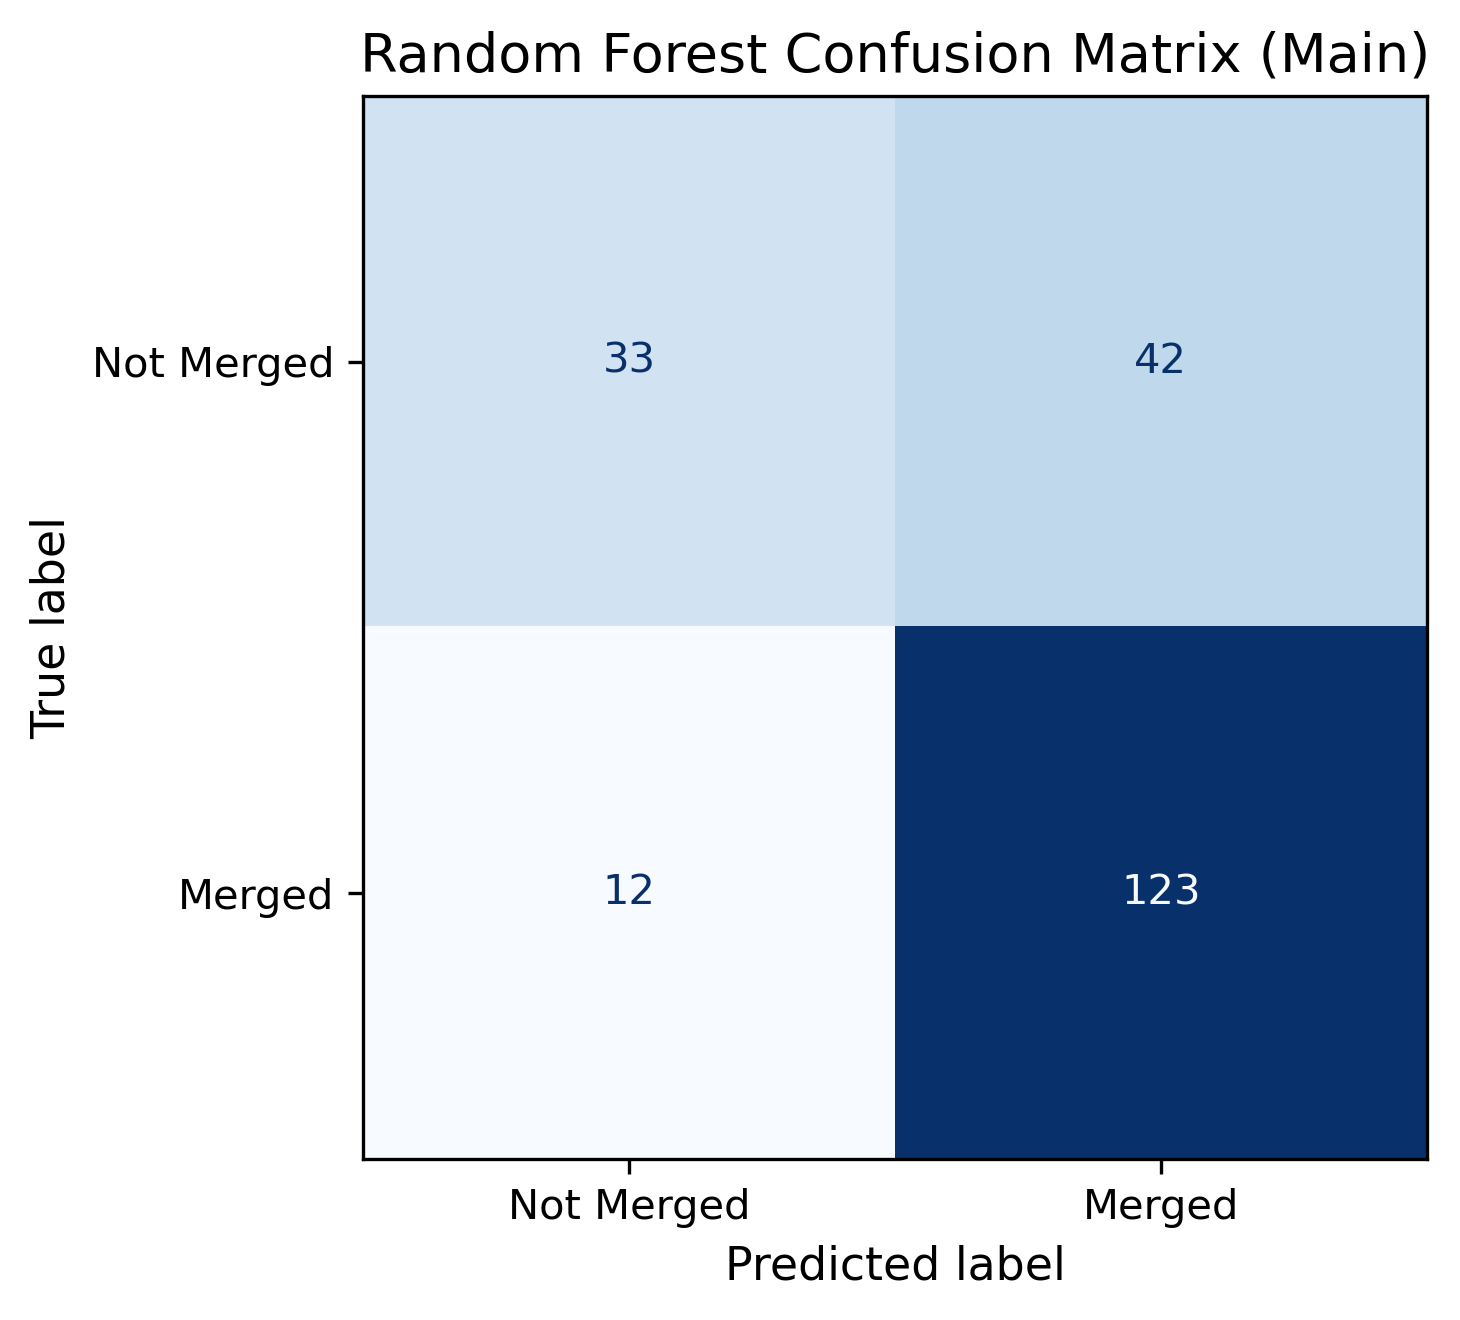
\includegraphics[width=0.48\textwidth]{../figures/07_confusion_matrix_rf.png}
\caption{SVM（左）与 Random Forest（右）混淆矩阵对比}
\end{figure}

\begin{figure}[ht]
\centering
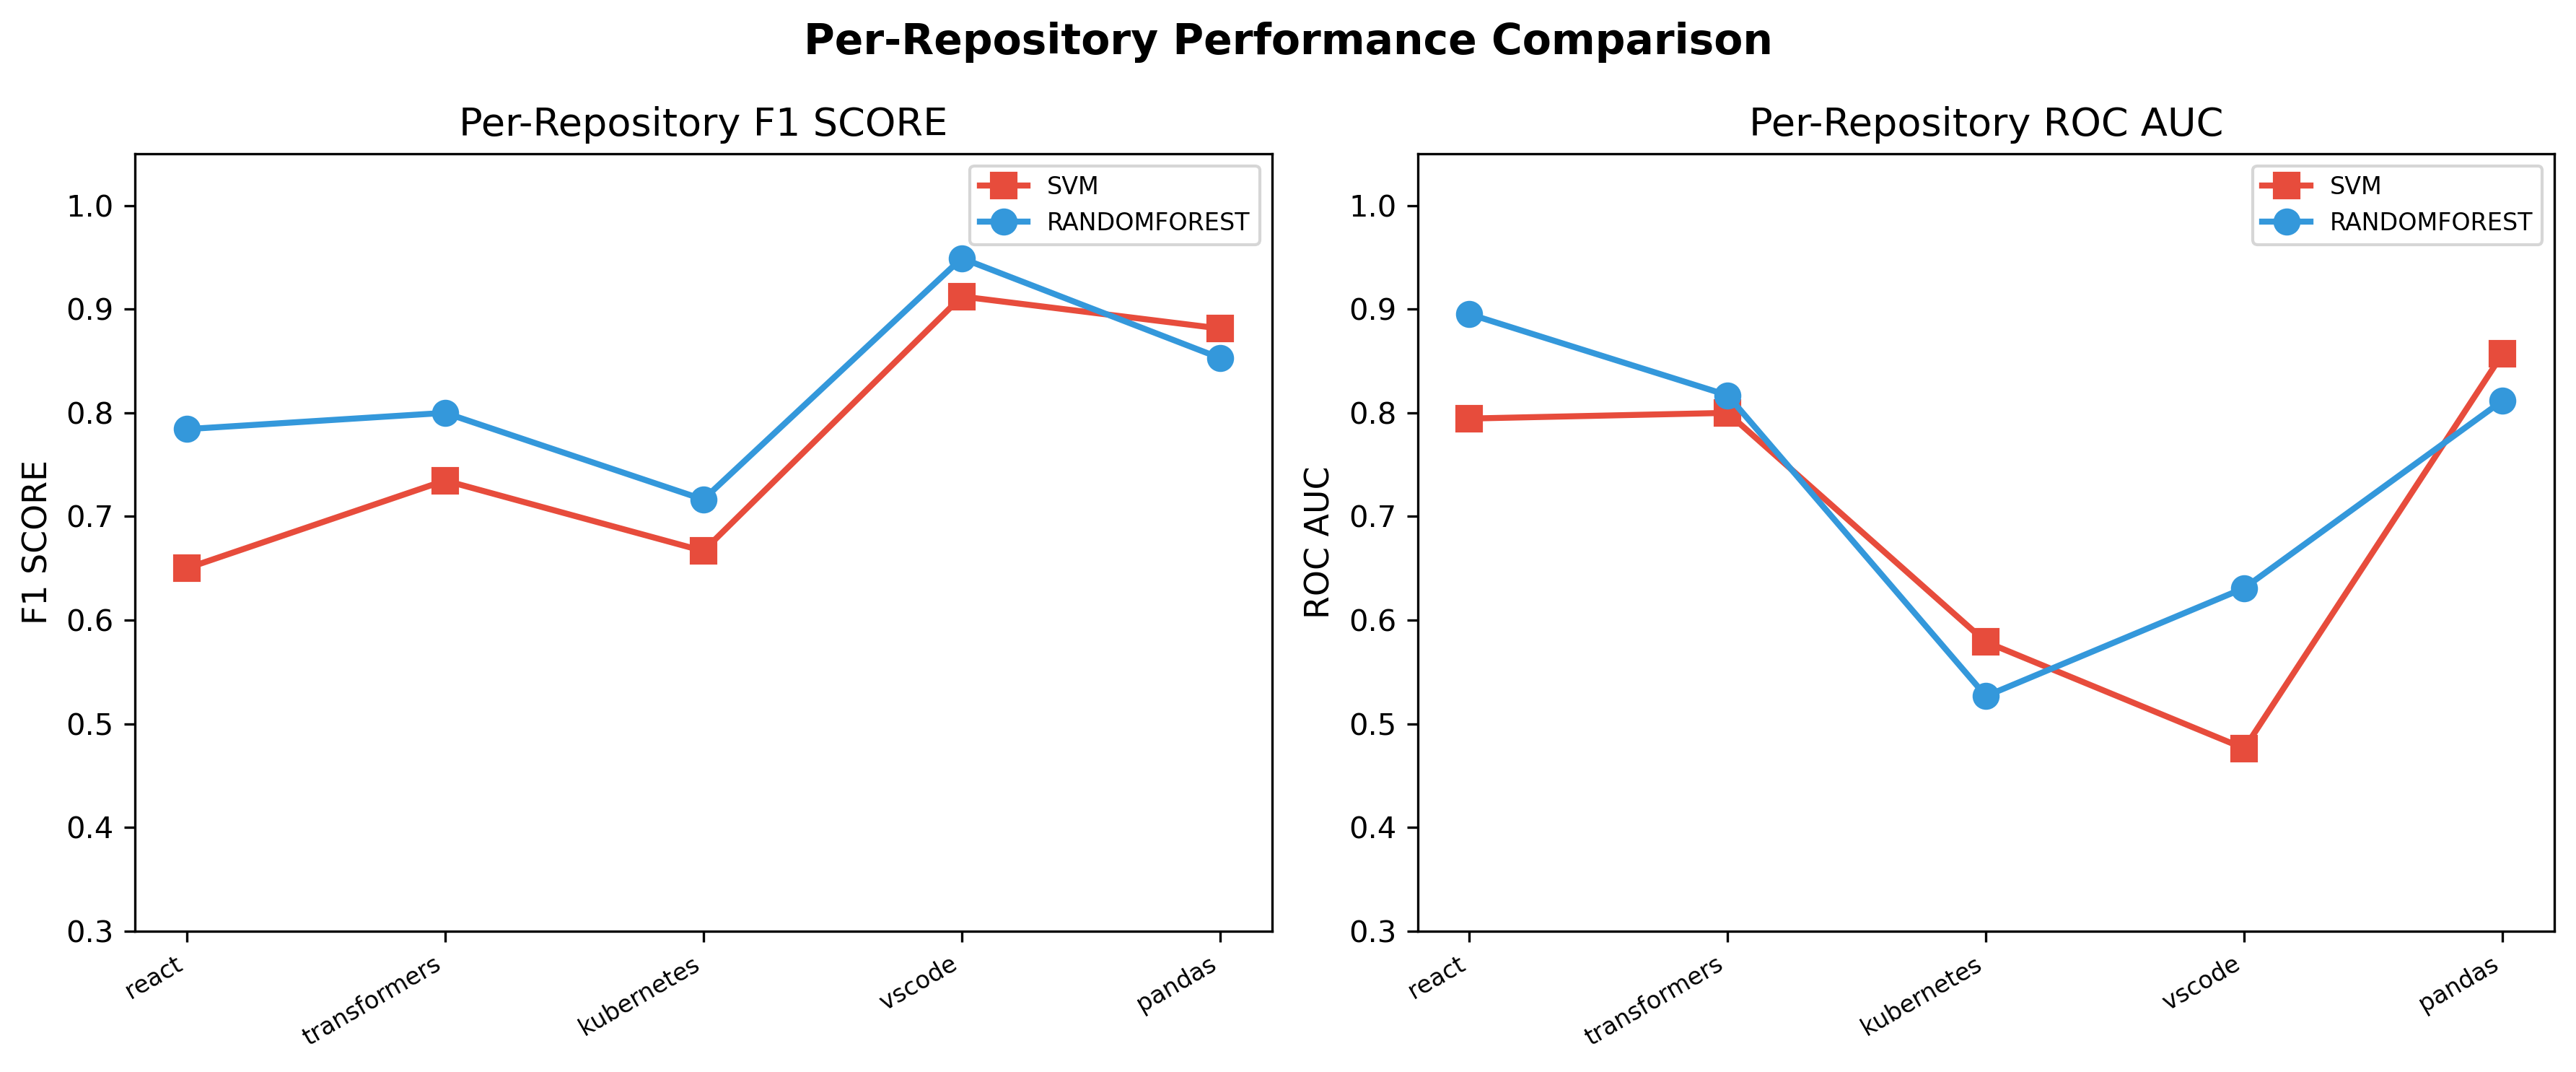
\includegraphics[width=\textwidth]{../figures/10_per_repo_performance.png}
\caption{分仓库 F1 与 ROC-AUC 对比}
\end{figure}

}
\clearpage
%========================
% 实验中遇到的问题
%========================

\experimentproblems{

\subsection*{4.1 为什么需要构建 AST 和 CFG 等代码中间表示？}

原始代码文本对机器学习模型而言是高维稀疏的，直接使用字符或词级别的特征难以捕捉程序的结构语义。AST 将代码转换为树形结构，保留了语法层次关系（如函数体嵌套在函数定义内）；CFG 将代码的执行路径建模为图结构，揭示了分支、循环和异常处理等控制流逻辑。这些中间表示将"文本"转换为"结构"，使模型能感知代码的复杂度和组织方式，从而提高预测能力。消融实验也验证了这一点：加入 AST 后 F1 从 0.8094 提升至 0.8227。

\subsection*{4.2 为什么传统机器学习需要人工设计特征？}

传统机器学习模型（SVM、Random Forest）接受固定长度的数值向量作为输入，本身不具备从原始文本或代码中自动学习表示的能力。因此需要人工将领域知识编码为特征，例如"修改了多少文件""AST 有多少层嵌套""描述有多少个词"。这与深度学习和大语言模型形成对比——后者可以通过神经网络自动从原始输入中学习表示，但代价是更高的训练成本、更大的参数量和更低的解释性。

\subsection*{4.3 SVM 和 Random Forest 分别适用于哪些应用场景？}

\textbf{SVM：}适用于中小规模数据集、特征维度较高的场景。通过核函数（如 RBF）可以处理非线性分类，对特征缩放敏感。SVM 的决策边界由支持向量决定，模型相对简洁。本实验中 SVM 的 Precision（0.8031）高于 RF（0.7455），适合对假阳性敏感的场合（如不希望误报一个 PR 会合并）。

\textbf{Random Forest：}适用于特征间存在复杂非线性关系的场景，对异常值和噪声更鲁棒，不需要特征缩放。RF 天然支持特征重要性评估和并行训练。本实验中 RF 的 Recall（0.9111）和整体 F1/AUC 均优于 SVM，更适合对召回率敏感的场景（如希望尽可能找出会合并的 PR）。

\subsection*{4.4 哪类特征对 Merge Prediction 贡献最大？为什么？}

实验结果显示，\textbf{文本特征}（PR 描述长度、Commit Message 长度）是最重要的预测因子（Top-5 中占 3 席），其次是\textbf{代码修改规模特征}（删除行数、新增行数）。

\textbf{原因分析：}
\begin{itemize}
    \item 高质量的 PR 描述和 Commit Message 反映了贡献者的认真程度和沟通能力，这与开源社区的代码审查文化高度一致——清晰的描述降低了审查者的理解成本，提高了合并意愿；
    \item 修改规模小、聚焦的 PR 更容易被审查者完整阅读和理解，审查周期短，合并概率高；
    \item AST/CFG 结构特征的贡献相对有限，主要是因为 patch 片段缺少完整的函数和文件上下文，结构特征的信息量天然受限。
\end{itemize}

\subsection*{4.5 与实验一相比，本实验的数据预处理增加了哪些步骤？}

实验一的数据预处理主要包括 API 数据采集、特征提取、统计分析。实验二在此基础上增加了：

\begin{enumerate}
    \item \textbf{数据筛选：}过滤 AI 生成代码 PR（97 条），删除异常样本（6 条 num\_changed\_files $\le$ 0），保留 1397 条人类代码 PR；
    \item \textbf{数据集划分：}按 repo + is\_merged 分层划分为 train/val/test（70/15/15），输出稳定的 splits.csv；
    \item \textbf{Patch 级代码提取：}从 raw JSON 的 Unified Diff 中提取新增代码行（约 225 万行），按文件类型分类；
    \item \textbf{AST/CFG 构建：}对代码文件进行 tree-sitter AST 解析和简化 CFG 构建，生成 23 个结构特征；
    \item \textbf{特征工程：}构建 61 维特征向量，包括派生特征（code\_churn、per\_file 指标）、文件类型分布、语言标记等，并进行 winsorize 截断和 StandardScaler 标准化；
    \item \textbf{信息泄漏控制：}主动排除审查决策、审阅者数量、标签等后验信息，仅使用 PR 提交时可获得的信息。
\end{enumerate}

\subsection*{4.6 实验中遇到的技术问题}

\textbf{（1）tree-sitter API 版本适配。} tree-sitter 0.26 的 Python API 与旧版本不同：Parser 构造需直接传入 Language 对象（而非先构造再 set\_language），且 tree-sitter-typescript 的语言函数命名为 \texttt{language\_typescript()} 和 \texttt{language\_tsx()} 而非统一的 \texttt{language()}。通过查阅官方文档和运行时反射（getattr）解决。

\textbf{（2）patch\_index.json 文件过大。} 初始方案存储了每个文件的新增代码行列表，JSON 缩进格式下文件达 122 MB。优化方案为：将代码行列表合并为单个字符串（用 \textbackslash n 连接），并使用紧凑 JSON（无缩进）序列化，最终压缩至 89.5 MB。

\textbf{（3）特征维度的差异导致评估阶段报错。} 可视化 ROC 曲线时，主实验模型（61 维特征）与上界实验模型（71 维特征）的输入维度不一致，若统一使用主实验特征文件加载会导致预测失败。解决方式是为每个实验加载对应的特征文件。

\textbf{（4）Kubernetes 仓库性能异常偏低。} 测试集上 Kubernetes 的 AUC 仅 0.5267，接近随机。排查发现 Kubernetes 的审查流程采用 SIG 机制和多阶段审查，PR 合并决策与代码修改特征的关联模式与其他仓库差异较大，属于仓库特异性问题，非数据泄漏或实现错误。

\textbf{（5）Scikit-learn 版本兼容性。} ConfusionMatrixDisplay.from\_predictions() 的参数名在不同版本中为 \texttt{display\_labels}（非 \texttt{display\_names}），需根据实际版本调整。

}

%========================
% 实验体会
%========================

\experimentexperience{

通过本实验，我对传统机器学习在代码审查任务中的应用有了系统的实践体验。从数据筛选到特征工程再到模型训练与评估，完整地走通了"原始数据 $\to$ 特征向量 $\to$ 分类模型"的标准流水线。

\textbf{主要收获：}

（1）\textbf{信息泄漏是实验设计中最需要警惕的问题。} 主实验与上界实验的对比清晰地表明：如果使用了审查结果特征，模型看似表现优异（AUC 0.95），但这是建立在后验信息上的"虚假繁荣"，实际部署时完全不可用。这一教训对后续所有实验（包括深度学习和 LLM 实验）都有重要指导意义。

（2）\textbf{传统机器学习的重要价值在于可解释性。} Random Forest 的特征重要性分析直观地告诉我们：PR 描述的质量和修改规模是决定合并与否的关键因素。这为后续实验六（Prompt 优化）和实验七（VSCode 插件）直接提供了设计方向——可以提示开发者完善 PR 描述、控制修改规模。

（3）\textbf{Patch 级别的代码分析有其固有局限。} AST/CFG 特征的边际贡献有限，不是特征工程的问题，而是数据本身的不完整性导致的——patch 只包含局部代码行，缺少完整文件上下文。这一发现为后续使用 Code2Vec、CodeBERT 等表示学习方法提供了有力的动机：深度模型或许能更好地从局部补丁中捕捉代码语义。

（4）\textbf{工程实践能力的提升。} 从 tree-sitter 多语言配置到 GridSearchCV 超参数搜索，从 patch\_index 的大文件优化到分仓库性能分析，本实验涵盖了数据科学项目中的多个实际挑战。

本实验产出的划分文件（splits.csv）、特征矩阵（features\_main.csv）和基线模型（SVM/RF）将作为实验三至七的比较基准，确保传统 ML、深度学习、LLM 方法在同一测试集上可公平对比。

}

%========================
% 教师评语
%========================

\teachercomment

\end{document}
